\documentclass[aspectratio=169,12pt]{beamer}
\usepackage[utf8]{inputenc}
\usepackage[T1]{fontenc}
\usepackage{amsmath, amssymb}
\usepackage{mathtools}
\DeclarePairedDelimiter{\ceil}{\lceil}{\rceil}
\usepackage{booktabs}
\usepackage{colortbl}
\usepackage{hyperref}
\usepackage{makecell}
\usepackage{ragged2e}
\usepackage{bytefield}
\usepackage{tikz}
\usetikzlibrary{arrows.meta, positioning, shapes.geometric, calc, tikzmark, shapes.misc, matrix, fit, backgrounds}
\usepackage{circuitikz}
\usepackage{tikz-timing}
\usepackage{tcolorbox}
\usepackage{minted}

\usetheme{Madrid}
\usecolortheme{default}

% Custom colors
\definecolor{mygreen}{RGB}{0,128,0}
\definecolor{myblue}{RGB}{0,0,255}
\definecolor{myred}{RGB}{255,0,0}

\title{System}
\author{Computer Architecture 2360267}
\date{2025, Lecture \#5}

% Clock macro - draws a clock at given location
\newcommand{\drawclock}[1]{
    \begin{scope}[shift={(#1)}]
        \draw[thick] (0,0) circle (0.12);
        \draw[thick] (0,0) -- (0,0.08);
        \draw[thick] (0,0) -- (0.05,-0.03);
    \end{scope}
}

% Hide macro - hides content by doing nothing with it
\newcommand{\hide}[1]{}

\begin{document}

\frame{\titlepage}

% Table of Contents
\begin{frame}{Outline}
\tableofcontents
\end{frame}

\section{CPU Architecture Overview}

% Slide 5: Putting It All Together
\begin{frame}{Hierarchy: From Transistor to System}
\begin{center}
\vspace{-1mm}
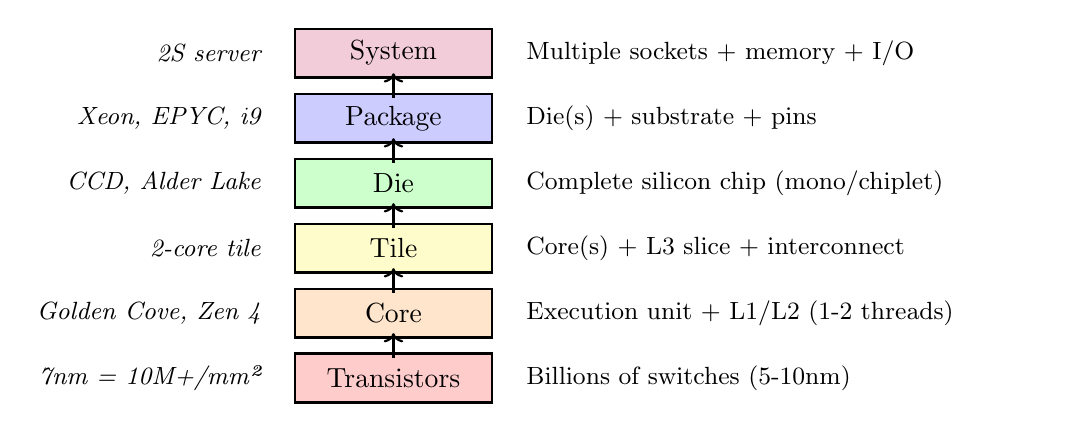
\begin{tikzpicture}[scale=0.75,
    level/.style={draw, thick, minimum width=2.5cm, minimum height=0.62cm, inner sep=1pt},
    desc/.style={text width=6.5cm, anchor=west, font=\small, align=left, inner ysep=0pt},
    example/.style={anchor=east, font=\small\itshape}
]

% Hierarchy levels
\node[level, fill=red!20] (trans) at (0,0) {Transistors};
\node[level, fill=orange!20] (core) at (0,1.1) {Core};
\node[level, fill=yellow!20] (tile) at (0,2.2) {Tile};
\node[level, fill=green!20] (die) at (0,3.3) {Die};
\node[level, fill=blue!20] (package) at (0,4.4) {Package};
\node[level, fill=purple!20] (system) at (0,5.5) {System};

% Descriptions - using style with reduced spacing
\node[desc] (trans_desc) at ([xshift=0.4cm]trans.east) {Billions of switches (5-10nm)};
\node[desc] at (trans_desc.west |- core) {Execution unit + L1/L2 (1-2 threads)};
\node[desc] at (trans_desc.west |- tile) {Core(s) + L3 slice + interconnect};
\node[desc] at (trans_desc.west |- die) {Complete silicon chip (mono/chiplet)};
\node[desc] at (trans_desc.west |- package) {Die(s) + substrate + pins};
\node[desc] at (trans_desc.west |- system) {Multiple sockets + memory + I/O};

% Examples on left - using style
\node[example] (trans_ex) at ([xshift=-0.4cm]trans.west) {7nm = 10M+/mm²};
\node[example] at (trans_ex.east |- core) {Golden Cove, Zen 4};
\node[example] at (trans_ex.east |- tile) {2-core tile};
\node[example] at (trans_ex.east |- die) {CCD, Alder Lake};
\node[example] at (trans_ex.east |- package) {Xeon, EPYC, i9};
\node[example] at (trans_ex.east |- system) {2S server};

% Arrows
\foreach \i in {0,1,2,3,4} {
    \draw[->, thick] (0,\i*1.1+0.34) -- (0,\i*1.1+0.76);
}

\end{tikzpicture}
\end{center}

\vspace{-2mm}
\textbf{Key Insight:} Each level has its own interconnect needs:
\begin{itemize}
\item Within core: Register bypass networks
\item Within tile: L2-L3 connections
\item Within die: Ring/mesh/crossbar
\item Within package: Die-to-die (chiplets)
\item Between packages: UPI/IF (NUMA)
\end{itemize}
\end{frame}
% Slide 1: Core vs Uncore
\begin{frame}{CPU Architecture: Core vs Uncore}
\begin{columns}[T]
\column{0.5\textwidth}
\textbf{\textcolor{blue}{Core} (Execution Core):}
\begin{itemize}
\item The \textbf{actual processing unit}
\item Contains:
  \begin{itemize}
  \item ALUs, FPU
  \item Registers
  \item L1 cache (I\$ + D\$)
  \item Usually L2 cache (\textbf{private})
  \item Branch predictor
  \item Decode/dispatch units
  \end{itemize}
\item Each core can run 1-2 threads (with SMT/HT)
\item The part that \textbf{executes instructions}
\end{itemize}

\column{0.5\textwidth}
\textbf{\textcolor{green!50!black}{Uncore} (System Agent):}
\begin{itemize}
\item \textbf{Everything else} on the chip
\item Contains:
  \begin{itemize}
  \item Memory controllers
  \item Last Level Cache (LLC/L3)
  \item PCIe controllers
  \item Interconnect (ring/mesh)
  \item Power management
  \item Integrated GPU (if present)
  \end{itemize}
\item \textbf{Shared by all cores}
\item Runs at different frequency (often lower)
\end{itemize}
\end{columns}
\end{frame}

% Slide 2: Tile Architecture
\begin{frame}{Tile Architecture}
\textbf{Tile}: A modular, repeatable unit in modern CPUs

\begin{columns}[T]
\column{0.5\textwidth}
\textbf{What's in a Tile:}
\begin{itemize}
\item One or two cores
\item Private L2 cache
\item Slice of shared L3 cache
\item Portion of the interconnect
\item Local routing/control logic
\end{itemize}

\vspace{0.3cm}
\textbf{Why Tiles?}
\begin{itemize}
\item Modular design (copy-paste)
\item Easier to scale (add more tiles)
\item Better yield (disable bad tiles)
\item Consistent layout for manufacturing
\end{itemize}

\column{0.5\textwidth}
\begin{center}
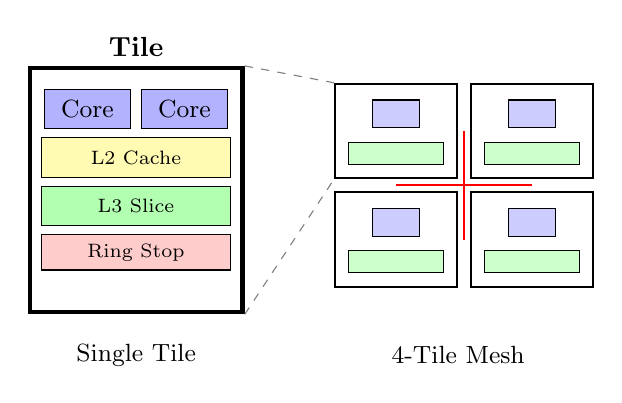
\begin{tikzpicture}[
    tilebox/.style={draw, ultra thick, minimum width=2.7cm, minimum height=3.1cm},
    corebox/.style={draw, fill=blue!30, minimum width=1.1cm, minimum height=0.5cm, inner sep=1pt, font=\small},
    cachebox/.style={draw, minimum width=2.4cm, minimum height=0.5cm, font=\scriptsize},
    minitile/.style={draw, thick, minimum width=1.55cm, minimum height=1.2cm}
]
% Single tile detail
\node[tilebox] (tile) at (0,0) {};
\node[font=\bfseries, anchor=south] at (tile.north) {Tile};
\node[corebox] (c1) at ([yshift=-0.55cm, xshift=-0.62cm]tile.north) {Core};
\node[corebox, right=0.12cm of c1] (c2) {Core};
\node[cachebox, fill=yellow!30, below=0.1cm of $(c1.south)!0.5!(c2.south)$] (l2) {L2 Cache};
\node[cachebox, fill=green!30, below=0.1cm of l2] (l3) {L3 Slice};
\node[cachebox, fill=red!20, below=0.1cm of l3, minimum height=0.3cm] (ring) {Ring Stop};
\node[font=\small, below=0.25cm of tile] (singlelabel) {Single Tile};

% Multiple tiles - 2x2 grid, positioned to the right
\node[minitile] (t00) at (3.3,0.75) {};
\node[minitile, right=0.15cm of t00] (t10) {};
\node[minitile, below=0.15cm of t00] (t01) {};
\node[minitile, right=0.15cm of t01] (t11) {};

% Mini content in each tile
\foreach \t in {t00,t10,t01,t11} {
    \node[draw, fill=blue!20, minimum width=0.6cm, minimum height=0.35cm] at ([yshift=0.22cm]\t.center) {};
    \node[draw, fill=green!20, minimum width=1.2cm, minimum height=0.28cm] at ([yshift=-0.28cm]\t.center) {};
}

% Mesh interconnect lines
\draw[red, thick] ($(t00.south)!0.5!(t01.north)$) -- ($(t10.south)!0.5!(t11.north)$);
\draw[red, thick] ($(t00.east)!0.5!(t10.west)$) -- ($(t01.east)!0.5!(t11.west)$);

% Zoom lines from Single Tile to top-left tile
\draw[dashed, gray] (tile.north east) -- (t00.north west);
\draw[dashed, gray] (tile.south east) -- (t00.south west);

% Label aligned with Single Tile using -|
\node[font=\small] at (singlelabel.center -| t01.south east) {4-Tile Mesh};
\end{tikzpicture}
\end{center}

\textbf{Examples:} Intel Skylake-SP (mesh), Lakefield (big+small), Server CPUs (10-40 tiles)
\end{columns}
\end{frame}

% Slide 1: Modern CPU Architecture Overview
\begin{frame}{Modern Multi-Core CPU Architecture}
\begin{columns}[T]
\column{0.55\textwidth}
\textbf{Hierarchy of Components:}
\begin{enumerate}
\item \textbf{Core}: Execution units + L1/L2 cache
\item \textbf{Socket/Package}: Multiple cores + shared L3 + memory controller
\item \textbf{System}: Multiple sockets + memory
\end{enumerate}

\vspace{0.3cm}
\textbf{Two Types of Interconnects:}
\begin{itemize}
\item \textcolor{blue}{\textbf{Intra-socket}}: Connects cores within CPU
\item \textcolor{red}{\textbf{Inter-socket}}: Connects different CPUs
\end{itemize}

\column{0.45\textwidth}
\begin{center}
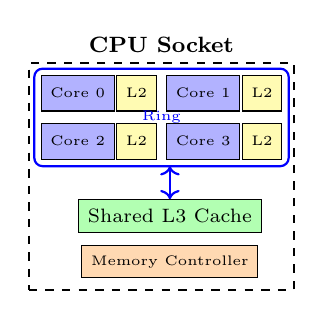
\begin{tikzpicture}[
    coreunit/.style={draw, fill=blue!30, minimum width=0.6cm, minimum height=0.45cm, text depth=0.1ex, font=\tiny},
    l2unit/.style={draw, fill=yellow!30, minimum width=0.4cm, minimum height=0.45cm, text depth=0.1ex, font=\tiny},
    l3box/.style={draw, fill=green!30, minimum height=0.4cm, text depth=0.1ex, font=\scriptsize},
    mcbox/.style={draw, fill=orange!30, minimum height=0.4cm, text depth=0.1ex, font=\tiny}
]
% Core 0 + L2 (top-left)
\node[coreunit] (c0) at (0,0) {Core 0};
\node[l2unit, right=0.02cm of c0] (l2c0) {L2};

% Core 1 + L2 (top-right)
\node[coreunit, right=0.12cm of l2c0] (c1) {Core 1};
\node[l2unit, right=0.02cm of c1] (l2c1) {L2};

% Core 2 + L2 (bottom-left)
\node[coreunit, below=0.15cm of c0] (c2) {Core 2};
\node[l2unit, right=0.02cm of c2] (l2c2) {L2};

% Core 3 + L2 (bottom-right)
\node[coreunit, right=0.12cm of l2c2] (c3) {Core 3};
\node[l2unit, right=0.02cm of c3] (l2c3) {L2};

% Ring interconnect - rectangle around cores
\draw[thick, blue, rounded corners=3pt]
    ([xshift=-0.08cm, yshift=0.08cm]c0.north west) --
    ([xshift=0.08cm, yshift=0.08cm]l2c1.north east) --
    ([xshift=0.08cm, yshift=-0.08cm]l2c3.south east) --
    ([xshift=-0.08cm, yshift=-0.08cm]c2.south west) -- cycle;
\node[blue, font=\tiny] at ($(l2c0.south east)!0.5!(c3.north west)$) {Ring};

% Shared L3 - further down
\node[l3box, below=0.5cm of $(c2.south)!0.5!(l2c3.south)$] (l3) {Shared L3 Cache};

% Memory Controller - centered below L3
\node[mcbox, below=0.15cm of l3] (mc) {Memory Controller};

% Connection from ring to L3
\draw[thick, blue, <->] ([yshift=-0.08cm]$(c2.south)!0.5!(l2c3.south)$) -- (l3.north);

% Socket container - fitted around content
\begin{scope}[on background layer]
\node[draw, thick, dashed, fit=(c0)(l2c1)(l3)(mc), inner sep=0.15cm] (socket) {};
\end{scope}
\node[font=\bfseries\footnotesize, anchor=south] at (socket.north) {CPU Socket};

\end{tikzpicture}
\end{center}
\end{columns}
\end{frame}
% Slide 2: Intra-Socket Interconnects
\begin{frame}{Intra-Socket Interconnects}
Connect cores, caches, memory controllers, and I/O within a single CPU package

\begin{center}
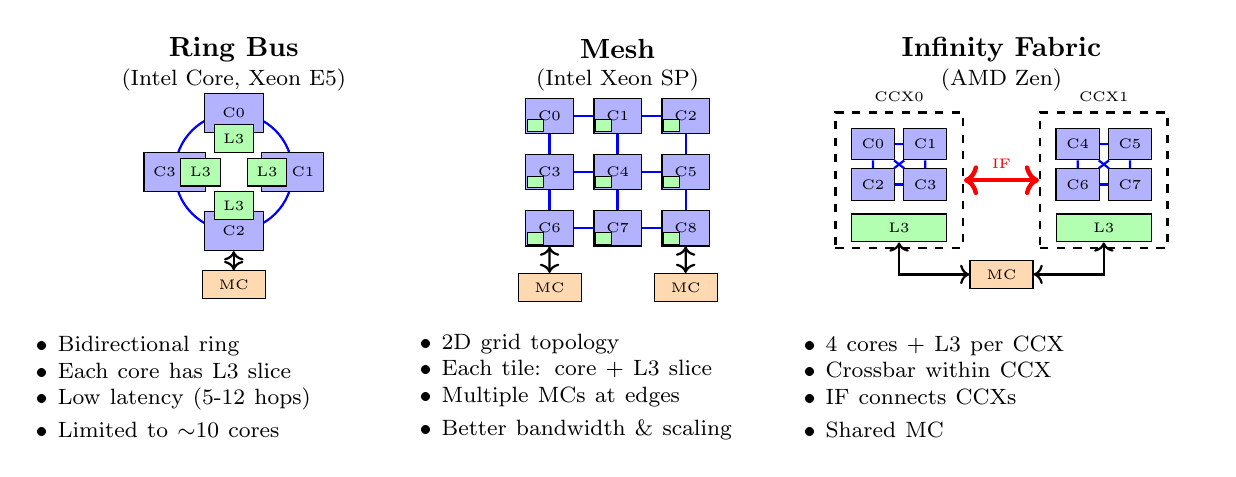
\begin{tikzpicture}[scale=0.65,
    core/.style={draw, rectangle, fill=blue!30, minimum width=0.75cm, minimum height=0.5cm, font=\tiny},
    corewide/.style={core, text width=0.55cm},
    cache/.style={draw, rectangle, fill=green!30, minimum width=2.5cm, minimum height=0.3cm},
    mc/.style={draw, rectangle, fill=orange!30, minimum width=0.8cm, minimum height=0.3cm}
]

% Ring Topology
\begin{scope}[shift={(-5,0)}]
\node at (0, 2.4) {\textbf{Ring Bus}};
\node at (0, 1.8) {\footnotesize (Intel Core, Xeon E5)};
% Draw ring - slightly larger
\draw[thick, blue] (0,0) circle (1.15cm);
% Add cores on the ring with visible numbers
\node[core] (c0) at (90:1.15) {C0};
\node[corewide, align=right] (c1) at (0:1.15) {C1};
\node[core] (c2) at (270:1.15) {C2};
\node[corewide, align=left] (c3) at (180:1.15) {C3};
% L3 slices inside the ring (shifted towards their cores)
\node[cache, minimum width=0.35cm, minimum height=0.22cm, font=\tiny] at (0,0.65) {L3};
\node[cache, minimum width=0.35cm, minimum height=0.22cm, font=\tiny] at (0.65,0) {L3};
\node[cache, minimum width=0.35cm, minimum height=0.22cm, font=\tiny] at (0,-0.65) {L3};
\node[cache, minimum width=0.35cm, minimum height=0.22cm, font=\tiny] at (-0.65,0) {L3};

\node[mc] (ring_mc) at (0,-2.2) {\tiny MC};
\draw[<->, thick] (c2) -- (ring_mc.north);

% Annotations
\node[text width=5cm, align=left] at (0,-4.2) {
\footnotesize
• Bidirectional ring\\
• Each core has L3 slice\\
• Low latency (5-12 hops)\\
• Limited to $\sim$10 cores
};
\end{scope}

% Mesh Topology
\begin{scope}[shift={(2.5,0)}]
\node at (0, 2.4) {\textbf{Mesh}};
\node at (0, 1.8) {\footnotesize (Intel Xeon SP)};
% Draw mesh as 3x3 matrix of cores
\matrix[matrix of nodes, nodes={core, minimum width=0.6cm, minimum height=0.45cm},
        row sep=0.25cm, column sep=0.25cm, ampersand replacement=\&] (mesh) {
    C0 \& C1 \& C2 \\
    C3 \& C4 \& C5 \\
    C6 \& C7 \& C8 \\
};
% Add small L3 slice inside each core
\foreach \i in {1,2,3} {
    \foreach \j in {1,2,3} {
        \node[fill=green!30, draw, minimum width=0.2cm, minimum height=0.15cm, inner sep=0, anchor=south west]
            at ([xshift=1pt, yshift=1pt]mesh-\i-\j.south west) {};
    }
}
% Draw mesh connections
\foreach \i in {1,2,3} {
    \draw[blue, thick] (mesh-\i-1.east) -- (mesh-\i-2.west);
    \draw[blue, thick] (mesh-\i-2.east) -- (mesh-\i-3.west);
}
\foreach \j in {1,2,3} {
    \draw[blue, thick] (mesh-1-\j.south) -- (mesh-2-\j.north);
    \draw[blue, thick] (mesh-2-\j.south) -- (mesh-3-\j.north);
}
\node[mc] (mesh_mc1) at ([yshift=-0.8cm]mesh-3-1.south) {\tiny MC};
\node[mc] (mesh_mc2) at ([yshift=-0.8cm]mesh-3-3.south) {\tiny MC};
\draw[<->, thick] (mesh-3-1.south) -- (mesh_mc1.north);
\draw[<->, thick] (mesh-3-3.south) -- (mesh_mc2.north);

% Annotations
\node[text width=5cm, align=left] at (0,-4.2) {
\footnotesize
• 2D grid topology\\
• Each tile: core + L3 slice\\
• Multiple MCs at edges\\
• Better bandwidth \& scaling
};
\end{scope}

% Crossbar/IF
\begin{scope}[shift={(10,0)}]
\node at (0, 2.4) {\textbf{Infinity Fabric}};
\node at (0, 1.8) {\footnotesize (AMD Zen)};

% CCX 0
\matrix[matrix of nodes, nodes={core, minimum width=0.55cm, minimum height=0.4cm},
        row sep=0.1cm, column sep=0.1cm, ampersand replacement=\&] (ccx0) at (-2.0,0.15) {
    C0 \& C1 \\
    C2 \& C3 \\
};
% Crossbar connections within CCX0
\draw[blue, thick] (ccx0-1-1) -- (ccx0-1-2);
\draw[blue, thick] (ccx0-1-1) -- (ccx0-2-1);
\draw[blue, thick] (ccx0-1-1) -- (ccx0-2-2);
\draw[blue, thick] (ccx0-1-2) -- (ccx0-2-1);
\draw[blue, thick] (ccx0-1-2) -- (ccx0-2-2);
\draw[blue, thick] (ccx0-2-1) -- (ccx0-2-2);
\node[cache, minimum width=1.2cm, minimum height=0.22cm, below=1pt of ccx0] (l3a) {\tiny L3};
\node[draw, dashed, thick, fit=(ccx0) (l3a), inner sep=2pt, label={[font=\tiny]above:CCX0}] (box0) {};

% CCX 1
\matrix[matrix of nodes, nodes={core, minimum width=0.55cm, minimum height=0.4cm},
        row sep=0.1cm, column sep=0.1cm, ampersand replacement=\&] (ccx1) at (2.0,0.15) {
    C4 \& C5 \\
    C6 \& C7 \\
};
% Crossbar connections within CCX1
\draw[blue, thick] (ccx1-1-1) -- (ccx1-1-2);
\draw[blue, thick] (ccx1-1-1) -- (ccx1-2-1);
\draw[blue, thick] (ccx1-1-1) -- (ccx1-2-2);
\draw[blue, thick] (ccx1-1-2) -- (ccx1-2-1);
\draw[blue, thick] (ccx1-1-2) -- (ccx1-2-2);
\draw[blue, thick] (ccx1-2-1) -- (ccx1-2-2);
\node[cache, minimum width=1.2cm, minimum height=0.22cm, below=1pt of ccx1] (l3b) {\tiny L3};
\node[draw, dashed, thick, fit=(ccx1) (l3b), inner sep=2pt, label={[font=\tiny]above:CCX1}] (box1) {};

% Infinity Fabric interconnect
\draw[<->, ultra thick, red] (box0.east) -- node[above, font=\tiny] {IF} (box1.west);

% Memory controller
\node[mc] (ifmc) at (0,-2) {\tiny MC};
\draw[<->, thick] (l3a.south) |- (ifmc.west);
\draw[<->, thick] (l3b.south) |- (ifmc.east);

% Annotations
\node[text width=5cm, align=left] at (0,-4.2) {
\footnotesize
• 4 cores + L3 per CCX\\
• Crossbar within CCX\\
• IF connects CCXs\\
• Shared MC
};
\end{scope}

\end{tikzpicture}
\end{center}

\footnotesize All cores can access all cache and memory controllers, but with varying latency
\end{frame}
% Slide 3: Die and Multi-Die Designs
\begin{frame}{Die and Multi-Die Designs}
\begin{columns}[T]
\column{0.5\textwidth}
\textbf{Die:} Single piece of silicon cut from wafer
\begin{itemize}
\item Contains transistors/circuits
\item Traditional: 1 die = 1 CPU
\end{itemize}

\textbf{Monolithic:} Everything on one die
\begin{itemize}
\item Simpler, lower latency
\item More expensive (yield issues)
\item Size limited by manufacturing
\end{itemize}

\textbf{Multi-Die (Chiplet):} Multiple smaller dies
\begin{itemize}
\item Connected in package
\item Better yield, mix-and-match
\item Higher latency between dies
\end{itemize}

\column{0.5\textwidth}
\begin{center}
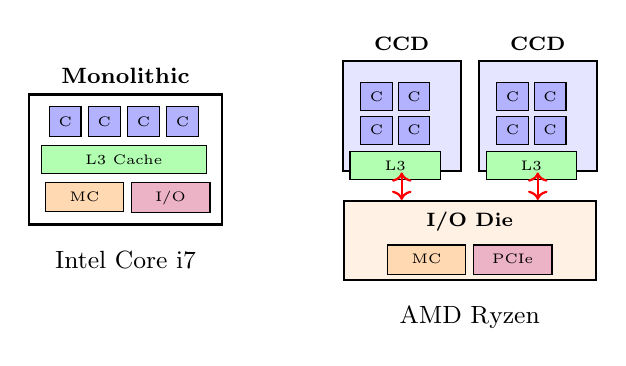
\begin{tikzpicture}[
    corebox/.style={draw, fill=blue!30, minimum width=0.38cm, minimum height=0.38cm, font=\tiny},
    minicore/.style={draw, fill=blue!30, minimum width=0.32cm, minimum height=0.32cm, font=\tiny},
    cachebox/.style={draw, fill=green!30, minimum height=0.3cm, font=\tiny},
    iobox/.style={draw, minimum width=1cm, minimum height=0.3cm, text depth=0.1ex, font=\tiny},
    ccdbox/.style={draw, thick, fill=blue!10, minimum width=1.5cm, minimum height=1.4cm},
    iodbox/.style={draw, thick, fill=orange!10, minimum width=3.2cm, minimum height=1cm}
]
% Monolithic - build from content outward
\node[corebox] (mc1) at (0,0) {C};
\node[corebox, right=0.08cm of mc1] (mc2) {C};
\node[corebox, right=0.08cm of mc2] (mc3) {C};
\node[corebox, right=0.08cm of mc3] (mc4) {C};
\node[cachebox, minimum width=2.1cm, below=0.1cm of $(mc1.south)!0.5!(mc4.south)$] (ml3) {L3 Cache};
\node[iobox, fill=orange!30, below=0.1cm of ml3, xshift=-0.5cm] (mmc) {MC};
\node[iobox, fill=purple!30, right=0.08cm of mmc] (mio) {I/O};

% Monolithic box fitted around content
\node[draw, thick, fit=(mc1)(mc4)(ml3)(mmc)(mio), inner sep=0.15cm] (mono) {};
\node[font=\footnotesize\bfseries, anchor=south] at (mono.north) {Monolithic};
\node[font=\small, below=0.2cm of mono] {Intel Core i7};

% Chiplet design - CCD 1
\node[ccdbox, right=1.5cm of mono, yshift=0.55cm] (ccd1) {};
\node[font=\scriptsize\bfseries, anchor=south] at (ccd1.north) {CCD};
\node[minicore] (cc1_1) at ([xshift=-0.32cm, yshift=0.25cm]ccd1.center) {C};
\node[minicore, right=0.06cm of cc1_1] (cc1_2) {C};
\node[minicore, below=0.06cm of cc1_1] (cc1_3) {C};
\node[minicore, right=0.06cm of cc1_3] (cc1_4) {C};
\node[cachebox, minimum width=1.15cm, below=0.08cm of $(cc1_3.south)!0.5!(cc1_4.south)$] (cl3_1) {L3};

% CCD 2
\node[ccdbox, right=0.2cm of ccd1] (ccd2) {};
\node[font=\scriptsize\bfseries, anchor=south] at (ccd2.north) {CCD};
\node[minicore] (cc2_1) at ([xshift=-0.32cm, yshift=0.25cm]ccd2.center) {C};
\node[minicore, right=0.06cm of cc2_1] (cc2_2) {C};
\node[minicore, below=0.06cm of cc2_1] (cc2_3) {C};
\node[minicore, right=0.06cm of cc2_3] (cc2_4) {C};
\node[cachebox, minimum width=1.15cm, below=0.08cm of $(cc2_3.south)!0.5!(cc2_4.south)$] (cl3_2) {L3};

% I/O Die
\node[iodbox, below=0.35cm of $(ccd1.south)!0.5!(ccd2.south)$] (iod) {};
\node[font=\scriptsize\bfseries, anchor=north] at ([yshift=-0.03cm]iod.north) {I/O Die};
\node[iobox, fill=orange!30, anchor=south, xshift=-0.55cm] at ([yshift=0.08cm]iod.south) (iomc) {MC};
\node[iobox, fill=purple!30, right=0.08cm of iomc] (iopcie) {PCIe};

% Connections
\draw[<->, red, thick] (ccd1.south) -- (ccd1.south |- iod.north);
\draw[<->, red, thick] (ccd2.south) -- (ccd2.south |- iod.north);

\node[font=\small, below=0.2cm of iod] {AMD Ryzen};
\end{tikzpicture}
\end{center}

\textbf{Chiplet Advantages:} Mix process nodes, reuse dies, better yields
\end{columns}
\end{frame}

% Slide 4: Package and Socket
\begin{frame}{Package and Socket}
\begin{columns}[T]
\column{0.5\textwidth}
\vspace{-3mm}
\textbf{Package:}
\begin{itemize}
\item Physical chip you can hold
\item Contains:
  \begin{itemize}
  \item One or more dies
  \item Substrate (PCB)
  \item Heat spreader (IHS)
  \item Pins/pads for connection
  \end{itemize}
\item Protects silicon
\item Provides electrical connections
\end{itemize}

\vspace{1mm}
\textbf{Socket:}
\begin{itemize}
\item Receptacle on motherboard
\item Holds the package
\item Examples: LGA1700, AM5, SP3
\item Defines:
  \begin{itemize}
  \item Pin count and layout
  \item Power delivery
  \item Memory channels
  \end{itemize}
\end{itemize}

\column{0.5\textwidth}
\vspace{-7mm}
\begin{center}
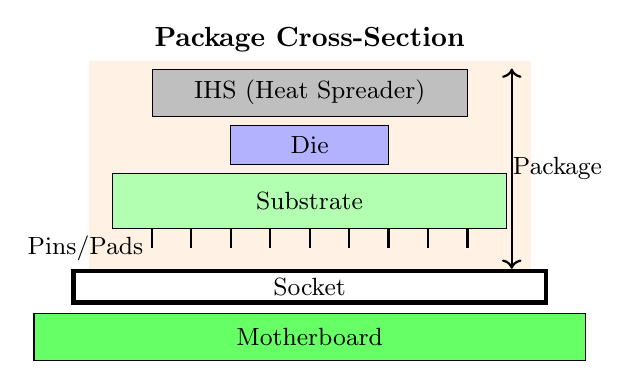
\begin{tikzpicture}[scale=0.8,
    every node/.style={inner sep=0pt},
    box/.style={draw, minimum height=6mm}]

% Motherboard (anchor element)
\node[box, minimum width=7cm, fill=green!60] (mobo) {\small Motherboard};

% Socket - above motherboard (text inside)
\node[box, minimum width=6cm, ultra thick, minimum height=4mm, above=1mm of mobo, inner sep=2pt] (socket) {\small Socket};

% Substrate - positioned above socket with space for pins
\node[box, minimum width=5cm, fill=green!30, minimum height=7mm, above=5mm of socket] (substrate) {\small Substrate};

% Pins - drawn from substrate bottom using calc
\foreach \i in {1,...,9} {
    \draw[thick] ($(substrate.south west)!{\i/10}!(substrate.south east)$) -- ++(0,-3mm);
}
\node[anchor=north east] at ([yshift=-1mm, xshift=5mm]substrate.south west) {\small Pins/Pads};

% Die - above substrate (narrower)
\node[box, minimum width=2cm, fill=blue!30, minimum height=5mm, above=1mm of substrate] (die) {\small Die};

% IHS (Heat Spreader) - above die
\node[box, minimum width=4cm, fill=gray!50, above=1mm of die] (ihs) {\small IHS (Heat Spreader)};

% Title - above IHS
\node[above=2mm of ihs] {\textbf{Package Cross-Section}};

% Package background shading using fit
\begin{scope}[on background layer]
    \node[fit=(ihs)(substrate), fill=orange!10, inner sep=3mm, yshift=-2mm] (package-bg) {};
\end{scope}

% Package arrow - right of diagram, using relative positioning
\coordinate (arrow-x) at ([xshift=7mm]ihs.north east);
\draw[<->, thick] (arrow-x |- ihs.north) -- (arrow-x |- socket.north) node[midway, right] {\small Package};
\end{tikzpicture}
\end{center}

\vspace{-3mm}
\textbf{Multi-Socket Systems:}
\begin{itemize}
\item 2S, 4S, 8S (S = Socket)
\item Each socket = independent CPU
\item Connected via UPI/IF
\item Creates NUMA topology
\end{itemize}
\end{columns}
\end{frame}




\section{Interconnects and Multi-Core Systems}




% Slide 6: Software Implications
\begin{frame}{Software Implications}
\begin{columns}[T]
\column{0.5\textwidth}
\textbf{Cache Coherency}
\begin{itemize}
\item Maintained automatically
\item But costs performance
\item Worse across sockets
\end{itemize}

\vspace{0.2cm}
\textbf{Memory Allocation}
\begin{itemize}
\item First-touch policy
\item NUMA-aware allocation
\item Thread-local storage
\end{itemize}

\vspace{0.2cm}
\textbf{Thread Placement}
\begin{itemize}
\item Pin threads to cores
\item Keep related threads on same socket
\item Minimize cross-socket communication
\end{itemize}

\column{0.5\textwidth}
\textbf{Performance Tips:}
\begin{itemize}
\item \textbf{Check your topology:}\\
   \texttt{lscpu -e} or \texttt{lstopo}

\item \textbf{Quick improvement:}\\
   \texttt{numactl --cpunodebind=0 ./app}

\item \textbf{For shared data:}\\
   Place on socket with most accessors

\item \textbf{For partitioned data:}\\
   Align partitions to NUMA nodes
\end{itemize}

\vspace{0.3cm}
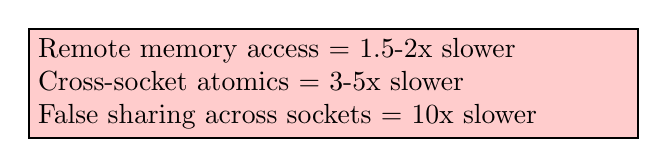
\begin{tikzpicture}
\node[draw, thick, fill=red!20, text width=7.5cm] at (0,0) {
%\textbf{Remember:}\\
Remote memory access = 1.5-2x slower\\
Cross-socket atomics = 3-5x slower\\
False sharing across sockets = 10x slower
};
\end{tikzpicture}
\end{columns}
\end{frame}


\section{NUMA Architecture}

% Slide: Multi-Processor Systems Introduction
\begin{frame}{Multi-Processor Systems}
\textbf{Why Multiple Processors?}
\begin{itemize}
\item Parallelizable complex tasks
\item Multiple tasks and/or multiple users
\item Performance scaling beyond single-core limits
\end{itemize}

\vspace{0.3cm}
\textbf{The Scaling Challenge:}
\begin{itemize}
\item Adding processors $\rightarrow$ memory becomes bottleneck
\item How processors access memory defines the architecture
\end{itemize}

\vspace{0.3cm}
\textbf{Memory Architecture Spectrum:}
\begin{center}
\footnotesize
\begin{tabular}{lccc}
\toprule
& \textbf{UMA} & \textbf{NUMA} & \textbf{Message Passing} \\
\midrule
Address Space & Shared & Shared & Private \\
Memory Access & Uniform & Non-uniform & Local only \\
Scalability & Low & Medium & High \\
Programming & Easy & Medium & Hard \\
\bottomrule
\end{tabular}
\end{center}
\end{frame}
% Slide: Multi-Processor Memory - UMA
\begin{frame}{Multi-Processor Memory: UMA}
\begin{columns}[T]
\column{0.55\textwidth}
\textbf{Uniform Memory Access (UMA)}
\begin{itemize}
\item Centralized shared memory
\item All processors access memory at similar latency
\item Simple programming model
\item Hardware maintains coherence (snooping)
\end{itemize}

\vspace{0.3cm}
\textbf{Scaling Limitation:}
\begin{itemize}
\item Shared bus $\rightarrow$ bandwidth bottleneck
\item Typically limited to 2--8 processors
\item $\Rightarrow$ Need distributed memory for more
\end{itemize}

\column{0.45\textwidth}
\begin{center}
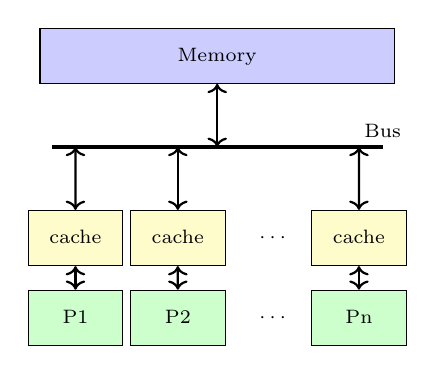
\begin{tikzpicture}[scale=0.7,
    comp/.style={draw, minimum height=7mm, minimum width=12mm, font=\scriptsize, text depth=0.5ex, text height=1.5ex},
    mem/.style={comp, fill=blue!20},
    cache/.style={comp, fill=yellow!20},
    proc/.style={comp, fill=green!20}]

% Memory at top (wide)
\node[mem, minimum width=4.5cm] (memory) {Memory};

% System bus - below memory (define as coordinate for -| usage)
\coordinate[below=8mm of memory] (bus-line);
\draw[ultra thick] ([xshift=-3cm]bus-line) coordinate (bus-left)
                -- ([xshift=3cm]bus-line) coordinate (bus-right);
\node[above, font=\scriptsize] at (bus-right) {Bus};

% Processor 1 (left)
\node[cache, below=8mm of bus-line, xshift=-1.8cm] (cache1) {cache};
\node[proc, below=3mm of cache1] (p1) {P1};

% Processor 2 (center-left)
\node[cache, below=8mm of bus-line, xshift=-0.5cm] (cache2) {cache};
\node[proc, below=3mm of cache2] (p2) {P2};

% Dots between P2 and Pn
\node[right=3mm of cache2, font=\scriptsize] {$\cdots$};
\node[right=3mm of p2, font=\scriptsize] {$\cdots$};

% Processor n (right)
\node[cache, below=8mm of bus-line, xshift=1.8cm] (cachen) {cache};
\node[proc, below=3mm of cachen] (pn) {Pn};

% Connection from memory to bus (vertical)
\draw[<->, thick] (memory) -- (bus-line -| memory);

% Connections from bus to caches (vertical using -|)
\draw[<->, thick] (bus-line -| cache1) -- (cache1);
\draw[<->, thick] (bus-line -| cache2) -- (cache2);
\draw[<->, thick] (bus-line -| cachen) -- (cachen);

% Connections from caches to processors
\draw[<->, thick] (cache1) -- (p1);
\draw[<->, thick] (cache2) -- (p2);
\draw[<->, thick] (cachen) -- (pn);

\end{tikzpicture}
\end{center}
\end{columns}
\end{frame}
% Slide: Multi-Processor Memory - NUMA
\begin{frame}{Multi-Processor Memory: NUMA}
\begin{columns}[T]
\column{0.55\textwidth}
\textbf{Non-Uniform Memory Access (NUMA)}

\smallskip
\textit{Solution: distribute memory with processors}

\begin{itemize}
\item Each processor has local memory
\item Still shared address space (DSM)
\item Variable latency:
  \begin{itemize}
  \item Local: fast
  \item Remote: via interconnect
  \end{itemize}
\item Scales to 100s of processors
\item Coherence:
  \begin{itemize}
  \item ccNUMA: hardware-managed (common)
  \item ncNUMA: software-managed (rare)
  \end{itemize}
\end{itemize}

\column{0.45\textwidth}
\begin{center}
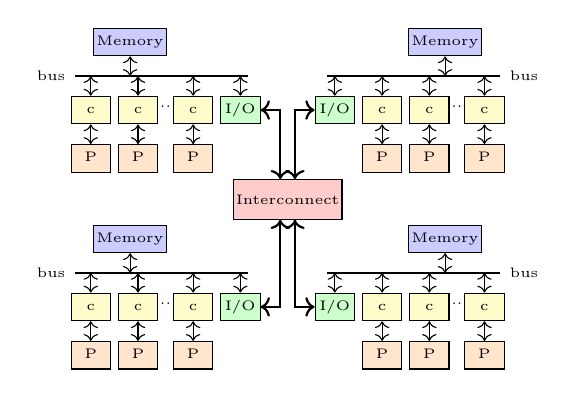
\begin{tikzpicture}[scale=0.5,
    % Compact styles for NUMA nodes
    scomp/.style={draw, minimum height=3.5mm, minimum width=5mm, font=\tiny, inner sep=1pt, text depth=0.2ex, text height=0.8ex},
    smem/.style={scomp, fill=blue!20},
    scache/.style={scomp, fill=yellow!20},
    sproc/.style={scomp, fill=orange!20},
    sio/.style={scomp, fill=green!20},
    % Pic for a NUMA node (I/O on right - for left-side nodes)
    pics/numanode/.style={code={
        \node[smem] (-mem) {Memory};
        \coordinate[below=2.5mm of -mem] (-bus);
        \draw[thick] ([xshift=-7mm]-bus) -- ([xshift=15mm]-bus);
        \node[left, font=\tiny] at ([xshift=-7mm]-bus) {bus};
        \draw[<->, thin] (-mem) -- (-bus);
        \node[scache, below=2.5mm of -bus, xshift=-5mm] (-c1) {\tiny c};
        \node[scache, below=2.5mm of -bus, xshift=1mm] (-c2) {\tiny c};
        \node[below=2.5mm of -bus, xshift=4.5mm, font=\tiny] {..};
        \node[scache, below=2.5mm of -bus, xshift=8mm] (-cn) {\tiny c};
        \node[sproc, below=2.5mm of -c1] (-p1) {\tiny P};
        \node[sproc, below=2.5mm of -c2] (-p2) {\tiny P};
        %\node[right=0mm of -p2, font=\tiny] {..};
        \node[sproc, below=2.5mm of -cn] (-pn) {\tiny P};
        \draw[<->, thin] (-bus -| -c1) -- (-c1);
        \draw[<->, thin] (-bus -| -c2) -- (-c2);
        \draw[<->, thin] (-bus -| -cn) -- (-cn);
        \draw[<->, thin] (-c1) -- (-p1);
        \draw[<->, thin] (-c2) -- (-p2);
        \draw[<->, thin] (-cn) -- (-pn);
        \node[sio, below=2.5mm of -bus, xshift=14mm] (-io) {I/O};
        \draw[<->, thin] (-bus -| -io) -- (-io);
    }},
    % Pic for a NUMA node (I/O on left - for right-side nodes)
    pics/numanodeR/.style={code={
        \node[smem] (-mem) {Memory};
        \coordinate[below=2.5mm of -mem] (-bus);
        \draw[thick] ([xshift=-15mm]-bus) -- ([xshift=7mm]-bus);
        \node[right, font=\tiny] at ([xshift=7mm]-bus) {bus};
        \draw[<->, thin] (-mem) -- (-bus);
        \node[sio, below=2.5mm of -bus, xshift=-14mm] (-io) {I/O};
        \node[scache, below=2.5mm of -bus, xshift=-8mm] (-c1) {\tiny c};
        \node[scache, below=2.5mm of -bus, xshift=-2mm] (-c2) {\tiny c};
        \node[below=2.5mm of -bus, xshift=1.5mm, font=\tiny] {..};
        \node[scache, below=2.5mm of -bus, xshift=5mm] (-cn) {\tiny c};
        \node[sproc, below=2.5mm of -c1] (-p1) {\tiny P};
        \node[sproc, below=2.5mm of -c2] (-p2) {\tiny P};
        \node[sproc, below=2.5mm of -cn] (-pn) {\tiny P};
        \draw[<->, thin] (-bus -| -io) -- (-io);
        \draw[<->, thin] (-bus -| -c1) -- (-c1);
        \draw[<->, thin] (-bus -| -c2) -- (-c2);
        \draw[<->, thin] (-bus -| -cn) -- (-cn);
        \draw[<->, thin] (-c1) -- (-p1);
        \draw[<->, thin] (-c2) -- (-p2);
        \draw[<->, thin] (-cn) -- (-pn);
    }}]

% Place 4 NUMA nodes (left nodes: I/O right, right nodes: I/O left)
\pic (n1) at (0,0) {numanode};
\pic (n2) at (8,0) {numanodeR};
\pic (n3) at (0,-5) {numanode};
\pic (n4) at (8,-5) {numanodeR};

% Central Interconnect
\node[draw, fill=red!20, minimum width=12mm, minimum height=5mm, font=\tiny, inner sep=1pt] (ic) at (4,-4) {Interconnect};

% Connect I/O to Interconnect
\draw[<->, thick] (n1-io.east) -| ([xshift=5mm]ic.north -| n1-io.east);
\draw[<->, thick] (n2-io.west) -| ([xshift=-5mm] ic.north -| n2-io.west);
\draw[<->, thick] (n3-io.east) -| ([xshift=5mm]ic.south -| n3-io.east);
\draw[<->, thick] (n4-io.west) -| ([xshift=-5mm]ic.south -| n4-io.west);

\end{tikzpicture}
\end{center}
\end{columns}
\end{frame}
% Slide: Multi-Processor Memory - Message Passing
\begin{frame}{Multi-Processor Memory: Message Passing}
\begin{columns}[T]
\column{0.55\textwidth}
\textbf{Message Passing (Clusters)}

\smallskip
\textit{Solution: give up shared address space}

\begin{itemize}
\item Each node: private memory only
\item No hardware coherence needed
\item Communication via explicit messages
  \begin{itemize}
  \item Send/Receive primitives
  \item e.g., MPI (Message Passing Interface)
  \end{itemize}
\item Scales to 1000s+ of nodes
\item Programming burden on software
\end{itemize}

\column{0.45\textwidth}
\begin{center}
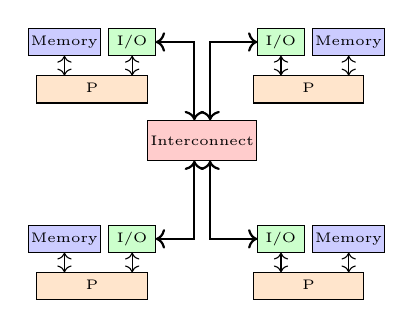
\begin{tikzpicture}[scale=0.5,
    % Same compact styles as NUMA
    scomp/.style={draw, minimum height=3.5mm, minimum width=6mm, font=\tiny, inner sep=1pt, outer sep=0pt, text depth=0.2ex, text height=0.8ex},
    smem/.style={scomp, fill=blue!20},
    sproc/.style={scomp, fill=orange!20, minimum width=14mm},
    sio/.style={scomp, fill=green!20},
    % Pic for message passing node (I/O on right - for left-side nodes)
    pics/mpnode/.style={code={
        \node[smem] (-mem) {Memory};
        \node[sio, right=1mm of -mem] (-io) {I/O};
        \node[sproc, below=2.5mm of -mem, xshift=3.5mm] (-p) {P};
        \draw[<->, thin] (-mem) -- (-mem |- -p.north);
        \draw[<->, thin] (-io) -- (-io |- -p.north);
    }},
    % Pic for message passing node (I/O on left - for right-side nodes)
    pics/mpnodeR/.style={code={
        \node[sio] (-io) {I/O};
        \node[smem, right=1mm of -io] (-mem) {Memory};
        \node[sproc, below=2.5mm of -io, xshift=3.5mm] (-p) {P};
        \draw[<->, thin] (-io) -- (-io |- -p.north);
        \draw[<->, thin] (-mem) -- (-mem |- -p.north);
    }}]

% Place 4 message passing nodes (2x2 layout)
\pic (n1) at (0,0) {mpnode};
\pic (n2) at (5.5,0) {mpnodeR};
\pic (n3) at (0,-5) {mpnode};
\pic (n4) at (5.5,-5) {mpnodeR};

% Central Interconnect (centered between left I/O and right I/O)
\node[draw, fill=red!20, minimum width=12mm, minimum height=5mm, font=\tiny, inner sep=1pt] (ic) at (3.5,-2.5) {Interconnect};

% Connect I/O to Interconnect
\draw[<->, thick] (n1-io.east) -| ([xshift=-2mm]ic.north);
\draw[<->, thick] (n2-io.west) -| ([xshift=2mm]ic.north);
\draw[<->, thick] (n3-io.east) -| ([xshift=-2mm]ic.south);
\draw[<->, thick] (n4-io.west) -| ([xshift=2mm]ic.south);

\end{tikzpicture}
\end{center}
\end{columns}
\end{frame}

% Slide: NUMA Topology
\begin{frame}{NUMA Node Topology}
\begin{columns}[T]
\column{0.45\textwidth}
\textbf{Key Concepts:}
\begin{itemize}
\item \textbf{NUMA Node}: CPU cores + local memory
\item \textbf{Socket}: Physical CPU package
\item \textbf{Distance}: Relative memory access cost
\item \textbf{Affinity}: Binding threads/memory to nodes
\end{itemize}

\vspace{0.3cm}
\textbf{Typical 2-Socket System:}
\begin{itemize}
\item Local memory: \textasciitilde100 cycles
\item Remote memory: \textasciitilde150-200 cycles
\item Can be 50-100\% slower!
\end{itemize}

\column{0.55\textwidth}
\begin{center}
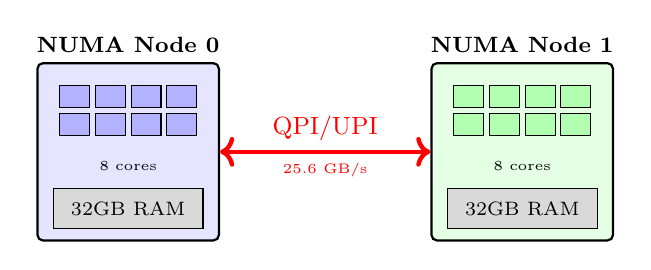
\begin{tikzpicture}[
    coreblue/.style={draw, fill=blue!30, minimum width=0.38cm, minimum height=0.28cm},
    coregreen/.style={draw, fill=green!30, minimum width=0.38cm, minimum height=0.28cm},
    ramblock/.style={draw, fill=gray!30, font=\scriptsize, minimum width=1.9cm, minimum height=0.5cm}
]
% NUMA Node 0 - cores as matrix at origin
\matrix[matrix of nodes, ampersand replacement=\&,
        nodes={coreblue}, row sep=0.06cm, column sep=0.06cm] (cores0) at (0,0) {
    \phantom{} \& \phantom{} \& \phantom{} \& \phantom{} \\
    \phantom{} \& \phantom{} \& \phantom{} \& \phantom{} \\
};
\node[font=\tiny, below=0.08cm of cores0] (lbl0) {8 cores};
\node[ramblock, below=0.1cm of lbl0] (ram0) {32GB RAM};

% NUMA Node 1 - cores as matrix, positioned relative to cores0
\matrix[matrix of nodes, ampersand replacement=\&,
        nodes={coregreen}, row sep=0.06cm, column sep=0.06cm,
        right=3.0cm of cores0] (cores1) {
    \phantom{} \& \phantom{} \& \phantom{} \& \phantom{} \\
    \phantom{} \& \phantom{} \& \phantom{} \& \phantom{} \\
};
\node[font=\tiny, below=0.08cm of cores1] (lbl1) {8 cores};
\node[ramblock, below=0.1cm of lbl1] (ram1) {32GB RAM};

% Background fit boxes
\begin{scope}[on background layer]
\node[draw, thick, fill=blue!10, rounded corners=2pt, fit=(cores0)(ram0), inner sep=0.15cm] (node0) {};
\node[draw, thick, fill=green!10, rounded corners=2pt, fit=(cores1)(ram1), inner sep=0.15cm] (node1) {};
\end{scope}

% Labels on top
\node[anchor=south, font=\footnotesize\bfseries] at (node0.north) {NUMA Node 0};
\node[anchor=south, font=\footnotesize\bfseries] at (node1.north) {NUMA Node 1};

% Interconnect
\draw[<->, ultra thick, red] (node0.east) -- node[above, font=\small] {QPI/UPI} node[below, font=\tiny] {25.6 GB/s} (node1.west);
\end{tikzpicture}
\end{center}

\begin{center}
\textbf{\small NUMA Distance Matrix}\\[0.1cm]
{\footnotesize Relative cost to access memory (10 = local)}\\[0.15cm]
\begin{tabular}{>{\footnotesize}r|>{\footnotesize}c>{\footnotesize}c}
node & 0 & 1 \\
\hline
0 & \textbf{10} & 21 \\
1 & 21 & \textbf{10} \\
\end{tabular}
\end{center}
\end{columns}
\end{frame}

% Slide 3: Interconnect Topologies
\begin{frame}{Interconnect Topologies}
\begin{center}
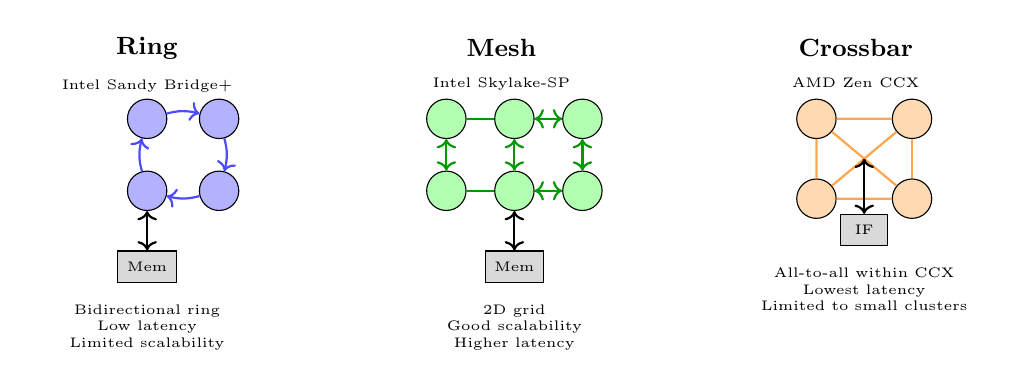
\begin{tikzpicture}[
    cpu/.style={draw, circle, minimum size=0.5cm, inner sep=1pt, font=\tiny},
    cpublue/.style={cpu, fill=blue!30},
    cpugreen/.style={cpu, fill=green!30},
    cpuorange/.style={cpu, fill=orange!30},
    mem/.style={draw, rectangle, fill=gray!30, minimum width=0.6cm, minimum height=0.4cm, font=\tiny},
    conn/.style={<->, thick},
    desc/.style={text width=2.8cm, align=center, font=\tiny}
]

% Ring (Intel)
\node (ringtitle) at (0, 1.4) {\small\textbf{Ring}};
\node[font=\tiny, below=0.02cm of ringtitle] {Intel Sandy Bridge+};
\node[cpublue] (r0) at (0,0.5) {};
\node[cpublue, right=0.4cm of r0] (r1) {};
\node[cpublue, below=0.4cm of r1] (r2) {};
\node[cpublue, left=0.4cm of r2] (r3) {};
\draw[->, thick, blue!70] (r0) to[bend left=15] (r1);
\draw[->, thick, blue!70] (r1) to[bend left=15] (r2);
\draw[->, thick, blue!70] (r2) to[bend left=15] (r3);
\draw[->, thick, blue!70] (r3) to[bend left=15] (r0);
\node[mem, below=0.5cm of r3] (rmem) {Mem};
\draw[conn] (r3) -- (rmem);
\node[desc, below=0.15cm of rmem] {Bidirectional ring\\ Low latency\\ Limited scalability};

% Mesh (Intel)
\node (meshtitle) at (4.5, 1.4) {\small\textbf{Mesh}};
\node[font=\tiny, below=0.02cm of meshtitle] {Intel Skylake-SP};
\node[cpugreen] (m00) at (3.8,0.5) {};
\node[cpugreen, right=0.35cm of m00] (m10) {};
\node[cpugreen, right=0.35cm of m10] (m20) {};
\node[cpugreen, below=0.4cm of m00] (m01) {};
\node[cpugreen, right=0.35cm of m01] (m11) {};
\node[cpugreen, right=0.35cm of m11] (m21) {};
\draw[conn, green!60!black] (m00) -- (m10) -- (m20);
\draw[conn, green!60!black] (m01) -- (m11) -- (m21);
\draw[conn, green!60!black] (m00) -- (m01);
\draw[conn, green!60!black] (m10) -- (m11);
\draw[conn, green!60!black] (m20) -- (m21);
\node[mem, below=0.5cm of m11] (mmem) {Mem};
\draw[conn] (m11) -- (mmem);
\node[desc, below=0.15cm of mmem] {2D grid\\ Good scalability\\ Higher latency};

% Crossbar (AMD)
\node (crosstitle) at (9, 1.4) {\small\textbf{Crossbar}};
\node[font=\tiny, below=0.02cm of crosstitle] {AMD Zen CCX};
\node[cpuorange] (x0) at (8.5,0.5) {};
\node[cpuorange, right=0.7cm of x0] (x1) {};
\node[cpuorange, below=0.5cm of x0] (x2) {};
\node[cpuorange, right=0.7cm of x2] (x3) {};
\draw[-, thick, orange!70] (x0) -- (x1) -- (x2) -- (x3) -- (x0) -- (x2);
\draw[-, thick, orange!70] (x1) -- (x3);
% IF connects to center of crossbar (shared L3/fabric)
\coordinate (xcenter) at ($(x0)!0.5!(x3)$);
\node[mem, below=0.7cm of xcenter] (xmem) {IF};
\draw[conn] (xcenter) -- (xmem);
\node[desc, below=0.15cm of xmem] {All-to-all within CCX\\ Lowest latency\\ Limited to small clusters};

\end{tikzpicture}
\end{center}

\textbf{Software Impact:}
\begin{itemize}
\item Different topologies $\rightarrow$ different performance characteristics
\item Ring: predictable latency, but can saturate with many cores
\item Mesh: better for many-core scaling, but more variable latency
\item Crossbar: excellent for small core counts, used in AMD's CCX design
\end{itemize}
\end{frame}

% Mesh Interconnect Detail
\begin{frame}{Mesh Interconnect (Intel Skylake-SP / Xeon Scalable)}
\begin{center}
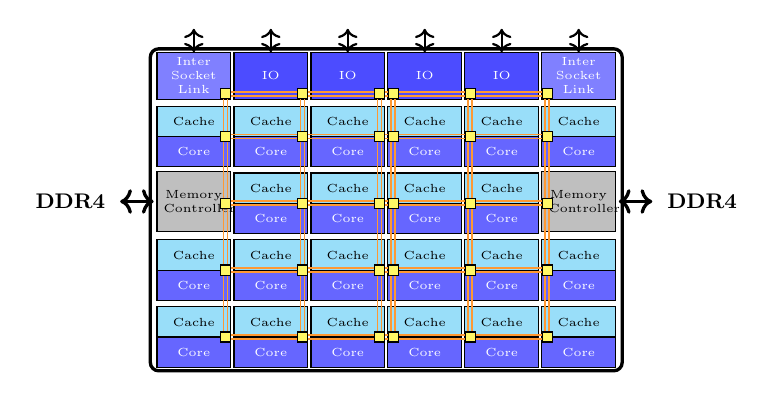
\begin{tikzpicture}[scale=0.85, transform shape,
    tile/.style={draw, minimum width=1.1cm, minimum height=0.45cm, font=\tiny, inner sep=1pt},
    iotile/.style={tile, fill=blue!70, text=white, minimum height=0.7cm},
    linktile/.style={tile, fill=blue!50, text=white, minimum height=0.7cm, text width=0.9cm, align=center},
    cachetile/.style={tile, fill=cyan!40},
    coretile/.style={tile, fill=blue!60, text=white},
    mctile/.style={tile, fill=gray!50, minimum height=0.9cm, text width=0.9cm, align=center},
    router/.style={draw, fill=yellow!60, minimum size=0.15cm, inner sep=0pt},
    meshline/.style={line width=0.5pt, orange!80},
    meshgap/.style={line width=0.04cm}
]

% Column positions (tighter spacing)
\def\colA{0}
\def\colB{1.15}
\def\colC{2.3}
\def\colD{3.45}
\def\colE{4.6}
\def\colF{5.75}

% Row positions (top to bottom) - rowI adjusted so IO/ISL has same gap to Cache as other rows
\def\rowI{-0.32}
\def\rowII{-1.0}
\def\rowIII{-2.0}
\def\rowIV{-3.0}
\def\rowV{-4.0}

% Top row: Inter Socket Link and IO
\node[linktile] at (\colA, \rowI) {Inter Socket Link};
\node[iotile] at (\colB, \rowI) {IO};
\node[iotile] at (\colC, \rowI) {IO};
\node[iotile] at (\colD, \rowI) {IO};
\node[iotile] at (\colE, \rowI) {IO};
\node[linktile] at (\colF, \rowI) {Inter Socket Link};

% Row 2: Cache + Core tiles
\foreach \col in {\colA, \colB, \colC, \colD, \colE, \colF} {
    \node[cachetile] at (\col, \rowII) {Cache};
    \node[coretile] at (\col, \rowII - 0.45) {Core};
}

% Row 3: Memory Controller on left, Cache+Core in middle, Memory Controller on right
\node[mctile] at (\colA, \rowIII - 0.2) {Memory\\Controller};
\foreach \col in {\colB, \colC, \colD, \colE} {
    \node[cachetile] at (\col, \rowIII) {Cache};
    \node[coretile] at (\col, \rowIII - 0.45) {Core};
}
\node[mctile] at (\colF, \rowIII - 0.2) {Memory\\Controller};

% Row 4: Cache + Core tiles
\foreach \col in {\colA, \colB, \colC, \colD, \colE, \colF} {
    \node[cachetile] at (\col, \rowIV) {Cache};
    \node[coretile] at (\col, \rowIV - 0.45) {Core};
}

% Row 5: Cache + Core tiles
\foreach \col in {\colA, \colB, \colC, \colD, \colE, \colF} {
    \node[cachetile] at (\col, \rowV) {Cache};
    \node[coretile] at (\col, \rowV - 0.45) {Core};
}

% Mesh line positions centered on router boxes
\def\tileHalfWidth{0.55}
\def\cacheCoreBoundary{-0.225}
\def\lineGap{0.03}
\def\routerHalf{0.075}  % half of router size (0.15cm)
\pgfmathsetmacro{\topRouterY}{\rowI - 0.35}

% Vertical mesh lines (double lines with arrows for bidirectional ring)
% Y coordinates: top router center to bottom router center (now at boundary)
\pgfmathsetmacro{\topCenterY}{\topRouterY + \routerHalf}
\pgfmathsetmacro{\bottomCenterY}{\rowV + \cacheCoreBoundary}
% Left 3 columns (A, B, C): lines centered on router (which is anchored at east edge)
\foreach \col in {\colA, \colB, \colC} {
    \pgfmathsetmacro{\lineX}{\col + \tileHalfWidth - \routerHalf}
    % One line going up (arrow at top), one going down (arrow at bottom)
    \draw[meshline, -{Stealth[length=1.5pt]}] (\lineX - \lineGap, \bottomCenterY) -- (\lineX - \lineGap, \topCenterY);
    \draw[meshline, -{Stealth[length=1.5pt]}] (\lineX + \lineGap, \topCenterY) -- (\lineX + \lineGap, \bottomCenterY);
}
% Right 3 columns (D, E, F): lines centered on router (which is anchored at west edge)
\foreach \col in {\colD, \colE, \colF} {
    \pgfmathsetmacro{\lineX}{\col - \tileHalfWidth + \routerHalf}
    \draw[meshline, -{Stealth[length=1.5pt]}] (\lineX - \lineGap, \bottomCenterY) -- (\lineX - \lineGap, \topCenterY);
    \draw[meshline, -{Stealth[length=1.5pt]}] (\lineX + \lineGap, \topCenterY) -- (\lineX + \lineGap, \bottomCenterY);
}

% Horizontal mesh lines (double lines with arrows for bidirectional ring)
\pgfmathsetmacro{\leftmostX}{\colA + \tileHalfWidth - \routerHalf}
\pgfmathsetmacro{\rightmostX}{\colF - \tileHalfWidth + \routerHalf}
% Top row horizontal line (router anchored at south, so center is up by routerHalf)
\pgfmathsetmacro{\topLineY}{\topRouterY + \routerHalf}
% One line going right (arrow at right), one going left (arrow at left)
\draw[meshline, -{Stealth[length=1.5pt]}] (\leftmostX, \topLineY - \lineGap) -- (\rightmostX, \topLineY - \lineGap);
\draw[meshline, -{Stealth[length=1.5pt]}] (\rightmostX, \topLineY + \lineGap) -- (\leftmostX, \topLineY + \lineGap);
% Cache/Core rows horizontal lines (router centered at boundary)
\foreach \row in {\rowII, \rowIII, \rowIV, \rowV} {
    \pgfmathsetmacro{\lineY}{\row + \cacheCoreBoundary}
    \draw[meshline, -{Stealth[length=1.5pt]}] (\leftmostX, \lineY - \lineGap) -- (\rightmostX, \lineY - \lineGap);
    \draw[meshline, -{Stealth[length=1.5pt]}] (\rightmostX, \lineY + \lineGap) -- (\leftmostX, \lineY + \lineGap);
}

% Routers at intersections
% Top row (IO/ISL) - anchored at SE corner for left cols, SW for right cols
% Tile half-width = 0.55, half-height = 0.35
\foreach \col in {\colA, \colB, \colC} {
    \pgfmathsetmacro{\rx}{\col + 0.55}
    \pgfmathsetmacro{\ry}{\rowI - 0.35}
    \node[router, anchor=south east] at (\rx, \ry) {};
}
\foreach \col in {\colD, \colE, \colF} {
    \pgfmathsetmacro{\rx}{\col - 0.55}
    \pgfmathsetmacro{\ry}{\rowI - 0.35}
    \node[router, anchor=south west] at (\rx, \ry) {};
}
% Cache/Core rows - centered on boundary between Cache and Core
\foreach \col in {\colA, \colB, \colC} {
    \foreach \row in {\rowII, \rowIII, \rowIV, \rowV} {
        \pgfmathsetmacro{\rx}{\col + 0.55}
        \pgfmathsetmacro{\ry}{\row - 0.225}
        \node[router, anchor=east] at (\rx, \ry) {};
    }
}
\foreach \col in {\colD, \colE, \colF} {
    \foreach \row in {\rowII, \rowIII, \rowIV, \rowV} {
        \pgfmathsetmacro{\rx}{\col - 0.55}
        \pgfmathsetmacro{\ry}{\row - 0.225}
        \node[router, anchor=west] at (\rx, \ry) {};
    }
}

% DDR4 arrows
\draw[<->, very thick] (-1.1, \rowIII - 0.2) -- (-0.6, \rowIII - 0.2);
\node[font=\small\bfseries, anchor=east] at (-1.2, \rowIII - 0.2) {DDR4};
\draw[<->, very thick] (6.35, \rowIII - 0.2) -- (6.85, \rowIII - 0.2);
\node[font=\small\bfseries, anchor=west] at (6.95, \rowIII - 0.2) {DDR4};

% Top arrows from IO/ISL tiles (extending further up)
\pgfmathsetmacro{\ioTop}{\rowI + 0.35}
\foreach \col in {\colA, \colB, \colC, \colD, \colE, \colF} {
    \draw[<->, thick] (\col, \ioTop + 0.35) -- (\col, \ioTop);
}

% Outer box - adjusted to fit tile positions
\pgfmathsetmacro{\boxTop}{\rowI + 0.4}
\pgfmathsetmacro{\boxBottom}{\rowV - 0.45 - 0.28}
\draw[very thick, rounded corners=3pt] (-0.65, \boxTop) rectangle (6.4, \boxBottom);

\end{tikzpicture}
\end{center}

\vspace{-0.2cm}
\begin{itemize}
\item Each tile: Core + private L1/L2 + slice of distributed L3 cache
\item Mesh routers at each intersection enable flexible routing
\item Memory controllers and I/O at edges; UPI links for multi-socket
\end{itemize}
\end{frame}

% Mesh Components - with overlays: 1=interconnect only, 2=with tiles
\begin{frame}{Mesh Components}
\begin{columns}[T]
\column{0.55\textwidth}
\begin{center}
\begin{tikzpicture}[scale=0.7, transform shape,
    tile/.style={draw, minimum width=0.9cm, minimum height=0.38cm, font=\tiny, inner sep=1pt},
    iotile/.style={tile, fill=blue!70, text=white, minimum height=0.55cm},
    linktile/.style={tile, fill=blue!50, text=white, minimum height=0.55cm, text width=0.75cm, align=center},
    cachetile/.style={tile, fill=cyan!40},
    coretile/.style={tile, fill=blue!60, text=white},
    mctile/.style={tile, fill=gray!50, minimum height=0.7cm, text width=0.75cm, align=center},
    router/.style={draw, fill=yellow!60, minimum size=0.12cm, inner sep=0pt},
    meshline/.style={line width=0.5pt, orange!80}
]

% Column and row positions
\def\colA{0}
\def\colB{0.95}
\def\colC{1.9}
\def\colD{2.85}
\def\colE{3.8}
\def\colF{4.75}
\def\rowI{-0.25}
\def\rowII{-0.85}
\def\rowIII{-1.65}
\def\rowIV{-2.45}
\def\rowV{-3.25}

\def\tileHalfWidth{0.45}
\def\cacheCoreBoundary{-0.19}
\def\lineGap{0.025}
\def\routerHalf{0.06}
\pgfmathsetmacro{\topRouterY}{\rowI - 0.275}
\pgfmathsetmacro{\topCenterY}{\topRouterY + \routerHalf}
\pgfmathsetmacro{\bottomCenterY}{\rowV + \cacheCoreBoundary}
\pgfmathsetmacro{\leftmostX}{\colA + \tileHalfWidth - \routerHalf}
\pgfmathsetmacro{\rightmostX}{\colF - \tileHalfWidth + \routerHalf}
\pgfmathsetmacro{\topLineY}{\topRouterY + \routerHalf}

% ===== ROUTERS FIRST (so lines draw on top) =====
\foreach \col in {\colA, \colB, \colC} {
    \node[router, anchor=south east] at (\col + 0.45, \rowI - 0.275) {};
}
\foreach \col in {\colD, \colE, \colF} {
    \node[router, anchor=south west] at (\col - 0.45, \rowI - 0.275) {};
}
\foreach \col in {\colA, \colB, \colC} {
    \foreach \row in {\rowII, \rowIII, \rowIV, \rowV} {
        \node[router, anchor=east] at (\col + 0.45, \row - 0.19) {};
    }
}
\foreach \col in {\colD, \colE, \colF} {
    \foreach \row in {\rowII, \rowIII, \rowIV, \rowV} {
        \node[router, anchor=west] at (\col - 0.45, \row - 0.19) {};
    }
}

% ===== MESH LINES (on top of routers, extended past edges) =====
\def\extendLen{0.15}  % How far lines extend past edge routers

% Vertical mesh lines - extended past top and bottom routers
\foreach \col in {\colA, \colB, \colC} {
    \pgfmathsetmacro{\lineX}{\col + \tileHalfWidth - \routerHalf}
    \draw[meshline] (\lineX - \lineGap, \bottomCenterY - \extendLen) -- (\lineX - \lineGap, \topCenterY + \extendLen);
    \draw[meshline] (\lineX + \lineGap, \bottomCenterY - \extendLen) -- (\lineX + \lineGap, \topCenterY + \extendLen);
}
\foreach \col in {\colD, \colE, \colF} {
    \pgfmathsetmacro{\lineX}{\col - \tileHalfWidth + \routerHalf}
    \draw[meshline] (\lineX - \lineGap, \bottomCenterY - \extendLen) -- (\lineX - \lineGap, \topCenterY + \extendLen);
    \draw[meshline] (\lineX + \lineGap, \bottomCenterY - \extendLen) -- (\lineX + \lineGap, \topCenterY + \extendLen);
}

% Horizontal mesh lines - extended past left and right routers
\draw[meshline] (\leftmostX - \extendLen, \topLineY - \lineGap) -- (\rightmostX + \extendLen, \topLineY - \lineGap);
\draw[meshline] (\leftmostX - \extendLen, \topLineY + \lineGap) -- (\rightmostX + \extendLen, \topLineY + \lineGap);
\foreach \row in {\rowII, \rowIII, \rowIV, \rowV} {
    \pgfmathsetmacro{\lineY}{\row + \cacheCoreBoundary}
    \draw[meshline] (\leftmostX - \extendLen, \lineY - \lineGap) -- (\rightmostX + \extendLen, \lineY - \lineGap);
    \draw[meshline] (\leftmostX - \extendLen, \lineY + \lineGap) -- (\rightmostX + \extendLen, \lineY + \lineGap);
}

% ===== TILES (only on slide 2) =====
\only<2>{
\node[linktile] at (\colA, \rowI) {Inter Socket Link};
\node[iotile] at (\colB, \rowI) {IO};
\node[iotile] at (\colC, \rowI) {IO};
\node[iotile] at (\colD, \rowI) {IO};
\node[iotile] at (\colE, \rowI) {IO};
\node[linktile] at (\colF, \rowI) {Inter Socket Link};

\foreach \col in {\colA, \colB, \colC, \colD, \colE, \colF} {
    \node[cachetile] at (\col, \rowII) {Cache};
    \node[coretile] at (\col, \rowII - 0.38) {Core};
}

\node[mctile] at (\colA, \rowIII - 0.15) {Mem\\Ctrl};
\foreach \col in {\colB, \colC, \colD, \colE} {
    \node[cachetile] at (\col, \rowIII) {Cache};
    \node[coretile] at (\col, \rowIII - 0.38) {Core};
}
\node[mctile] at (\colF, \rowIII - 0.15) {Mem\\Ctrl};

\foreach \col in {\colA, \colB, \colC, \colD, \colE, \colF} {
    \node[cachetile] at (\col, \rowIV) {Cache};
    \node[coretile] at (\col, \rowIV - 0.38) {Core};
    \node[cachetile] at (\col, \rowV) {Cache};
    \node[coretile] at (\col, \rowV - 0.38) {Core};
}

\draw[<->, thick] (-0.9, \rowIII - 0.15) -- (-0.5, \rowIII - 0.15);
\node[font=\tiny\bfseries, anchor=east] at (-0.95, \rowIII - 0.15) {DDR4};
\draw[<->, thick] (5.25, \rowIII - 0.15) -- (5.65, \rowIII - 0.15);
\node[font=\tiny\bfseries, anchor=west] at (5.7, \rowIII - 0.15) {DDR4};
}

% ===== RING CLOSURES (simple arcs) and ARROWS on straight lines =====
\pgfmathsetmacro{\topEndY}{\topCenterY + \extendLen}
\pgfmathsetmacro{\bottomEndY}{\bottomCenterY - \extendLen}
\pgfmathsetmacro{\leftEndX}{\leftmostX - \extendLen}
\pgfmathsetmacro{\rightEndX}{\rightmostX + \extendLen}
\def\arrowLen{0.08}

% Vertical ring closures (arcs) and vertical arrows
\foreach \col in {\colA, \colB, \colC} {
    \pgfmathsetmacro{\lineX}{\col + \tileHalfWidth - \routerHalf}
    % Top arc closure
    \draw[meshline] (\lineX - \lineGap, \topEndY) arc (180:0:\lineGap);
    % Bottom arc closure
    \draw[meshline] (\lineX + \lineGap, \bottomEndY) arc (0:-180:\lineGap);
    % Vertical arrows on extended lines (showing ring direction)
    \draw[meshline, -{Stealth[length=1.5pt]}] (\lineX - \lineGap, \topEndY - \arrowLen) -- (\lineX - \lineGap, \topEndY);
    \draw[meshline, -{Stealth[length=1.5pt]}] (\lineX + \lineGap, \topEndY) -- (\lineX + \lineGap, \topEndY - \arrowLen);
    \draw[meshline, -{Stealth[length=1.5pt]}] (\lineX + \lineGap, \bottomEndY + \arrowLen) -- (\lineX + \lineGap, \bottomEndY);
    \draw[meshline, -{Stealth[length=1.5pt]}] (\lineX - \lineGap, \bottomEndY) -- (\lineX - \lineGap, \bottomEndY + \arrowLen);
}
\foreach \col in {\colD, \colE, \colF} {
    \pgfmathsetmacro{\lineX}{\col - \tileHalfWidth + \routerHalf}
    % Top arc closure
    \draw[meshline] (\lineX - \lineGap, \topEndY) arc (180:0:\lineGap);
    % Bottom arc closure
    \draw[meshline] (\lineX + \lineGap, \bottomEndY) arc (0:-180:\lineGap);
    % Vertical arrows
    \draw[meshline, -{Stealth[length=1.5pt]}] (\lineX - \lineGap, \topEndY - \arrowLen) -- (\lineX - \lineGap, \topEndY);
    \draw[meshline, -{Stealth[length=1.5pt]}] (\lineX + \lineGap, \topEndY) -- (\lineX + \lineGap, \topEndY - \arrowLen);
    \draw[meshline, -{Stealth[length=1.5pt]}] (\lineX + \lineGap, \bottomEndY + \arrowLen) -- (\lineX + \lineGap, \bottomEndY);
    \draw[meshline, -{Stealth[length=1.5pt]}] (\lineX - \lineGap, \bottomEndY) -- (\lineX - \lineGap, \bottomEndY + \arrowLen);
}

% Horizontal ring closures (arcs) and horizontal arrows
\foreach \row in {\rowII, \rowIII, \rowIV, \rowV} {
    \pgfmathsetmacro{\lineY}{\row + \cacheCoreBoundary}
    % Left arc closure
    \draw[meshline] (\leftEndX, \lineY - \lineGap) arc (-90:-270:\lineGap);
    % Right arc closure
    \draw[meshline] (\rightEndX, \lineY + \lineGap) arc (90:-90:\lineGap);
    % Horizontal arrows
    \draw[meshline, -{Stealth[length=1.5pt]}] (\leftEndX + \arrowLen, \lineY - \lineGap) -- (\leftEndX, \lineY - \lineGap);
    \draw[meshline, -{Stealth[length=1.5pt]}] (\leftEndX, \lineY + \lineGap) -- (\leftEndX + \arrowLen, \lineY + \lineGap);
    \draw[meshline, -{Stealth[length=1.5pt]}] (\rightEndX - \arrowLen, \lineY + \lineGap) -- (\rightEndX, \lineY + \lineGap);
    \draw[meshline, -{Stealth[length=1.5pt]}] (\rightEndX, \lineY - \lineGap) -- (\rightEndX - \arrowLen, \lineY - \lineGap);
}
% Top row horizontal ring closures and arrows
\draw[meshline] (\leftEndX, \topLineY - \lineGap) arc (-90:-270:\lineGap);
\draw[meshline] (\rightEndX, \topLineY + \lineGap) arc (90:-90:\lineGap);
\draw[meshline, -{Stealth[length=1.5pt]}] (\leftEndX + \arrowLen, \topLineY - \lineGap) -- (\leftEndX, \topLineY - \lineGap);
\draw[meshline, -{Stealth[length=1.5pt]}] (\leftEndX, \topLineY + \lineGap) -- (\leftEndX + \arrowLen, \topLineY + \lineGap);
\draw[meshline, -{Stealth[length=1.5pt]}] (\rightEndX - \arrowLen, \topLineY + \lineGap) -- (\rightEndX, \topLineY + \lineGap);
\draw[meshline, -{Stealth[length=1.5pt]}] (\rightEndX, \topLineY - \lineGap) -- (\rightEndX - \arrowLen, \topLineY - \lineGap);

% Labels for slide 1
\only<1>{
\node[font=\scriptsize, orange!80] at (2.4, 0.5) {Horizontal Rings};
\node[font=\scriptsize, orange!80, rotate=90] at (5.6, -1.7) {Vertical Rings};
\node[font=\scriptsize, yellow!60!black] at (2.4, -4.0) {Mesh Stops (Routers)};
}

\end{tikzpicture}
\end{center}

\column{0.45\textwidth}
\only<1>{
\textbf{Mesh Fabric:}
\begin{itemize}
\item 2D array of bidirectional rings
\item Each column forms a vertical ring
\item Each row forms a horizontal ring
\item Mesh stops at intersections
\end{itemize}

\vspace{0.3cm}
\textbf{Why Mesh over Ring?}
\begin{itemize}
\item Ring limited to $\sim$10 cores
\item Mesh scales to 28+ cores
\item Better bandwidth \& latency
\end{itemize}
}
\only<2>{
\textbf{Tile Types:}
\begin{itemize}
\item \textbf{Core/LLC}: CPU + L3 slice
\item \textbf{Memory Ctrl}: DDR interface
\item \textbf{I/O}: PCIe, DMI
\item \textbf{Inter-Socket}: UPI link
\end{itemize}

\vspace{0.3cm}
\textbf{Mesh Stop (Router):}
\begin{itemize}
\item Interface: tile $\leftrightarrow$ fabric
\item Routes packets N/S/E/W
\item Handles coherency traffic
\end{itemize}
}
\end{columns}
\end{frame}

% Slide 4: Software Implications
\begin{frame}{NUMA: Software Implications}
\begin{columns}[T]
\column{0.5\textwidth}
\textbf{Performance Impact:}
\begin{itemize}
\item Remote memory access: 50-100\% slower
\item Cache coherency traffic across nodes
\item Memory bandwidth per node is limited
\item False sharing amplified across NUMA
\end{itemize}

\vspace{0.3cm}
\textbf{Common Issues:}
\begin{itemize}
\item Thread migration between nodes
\item Data allocated on "wrong" node
\item Unbalanced memory usage
\item Lock contention across nodes
\end{itemize}

\column{0.5\textwidth}
\textbf{Best Practices:}
\begin{enumerate}
\item \textbf{First-touch policy}: Allocate memory on the node that first accesses it
\item \textbf{Thread affinity}: Pin threads to specific cores/nodes
\item \textbf{Data partitioning}: Align data structures to NUMA boundaries
\item \textbf{NUMA-aware allocation}: Use \texttt{numa\_alloc\_onnode()}
\end{enumerate}

\vspace{0.3cm}
\textbf{Tools:}
\begin{itemize}
\item \texttt{numactl}: Control NUMA policy
\item \texttt{lstopo}: Visualize topology
\item \texttt{numastat}: Memory statistics
\item \texttt{perf}: Profile NUMA events
\end{itemize}
\end{columns}
\end{frame}

% Slide 5: NUMA Code Example
\begin{frame}[fragile]{NUMA-Aware Programming Example}
\begin{columns}[T]
\column{0.5\textwidth}
\textbf{NUMA-Unaware Code:}
\begin{tcolorbox}[colback=red!5!white, colframe=red!50!black, boxrule=0.5pt, left=1pt, right=1pt, top=1pt, bottom=1pt]
{\scriptsize
\begin{minted}{c}
// Thread 0 allocates all data
float* data = malloc(N * sizeof(float));

// All threads access same array
#pragma omp parallel
{
  int tid = omp_get_thread_num();
  int chunk = N / num_threads;
  int start = tid * chunk;

  // Remote memory access!
  for(int i = start; i < start+chunk; i++)
    data[i] = compute(i);
}
\end{minted}
}
\end{tcolorbox}

\column{0.5\textwidth}
\textbf{NUMA-Aware Code:}
\begin{tcolorbox}[colback=green!5!white, colframe=green!50!black, boxrule=0.5pt, left=1pt, right=1pt, top=1pt, bottom=1pt]
{\scriptsize
\begin{minted}{c}
#pragma omp parallel
{
  int tid = omp_get_thread_num();
  int chunk = N / num_threads;

  // Each thread allocates locally
  float* local_data =
    numa_alloc_local(chunk * sizeof(float));

  // Access local memory only
  for(int i = 0; i < chunk; i++)
    local_data[i] = compute(tid*chunk + i);

  // Copy to global if needed
  memcpy(&data[tid*chunk], local_data, ...);
}
\end{minted}
}
\end{tcolorbox}
\end{columns}

\vspace{0.3cm}
\textbf{Performance difference can be 2-3x for memory-bound workloads!}
\end{frame}

% Slide 6: Practical NUMA Considerations
\begin{frame}{Practical NUMA Considerations}
\begin{columns}[T]
\column{0.55\textwidth}
\textbf{When NUMA Matters Most:}
\begin{itemize}
\item Large working sets ($>$ L3 cache)
\item Memory-bandwidth intensive apps
\item Multi-socket servers
\item Database systems
\item Scientific computing (HPC)
\item In-memory key-value stores
\end{itemize}

\vspace{0.3cm}
\textbf{Quick Checks:}
\begin{itemize}
\item \texttt{lscpu | grep NUMA} - see topology
\item \texttt{numactl --hardware} - detailed info
\item \texttt{likwid-topology} - visual layout
\end{itemize}

\column{0.45\textwidth}
\begin{center}
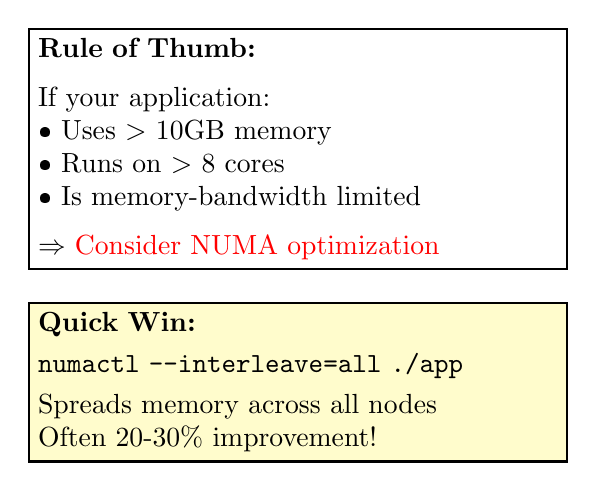
\begin{tikzpicture}[scale=0.8]
\node[text width=6.6cm, draw, thick] (rulethumb) at (0,0) {
\textbf{Rule of Thumb:}\\[0.2cm]
If your application:\\
• Uses $>$ 10GB memory\\
• Runs on $>$ 8 cores\\
• Is memory-bandwidth limited\\[0.2cm]
$\Rightarrow$ \textcolor{red}{Consider NUMA optimization}
};

\node[text width=6.6cm, draw, thick, fill=yellow!20, anchor=north] at ([yshift=-0.5cm]rulethumb.south) {
\textbf{Quick Win:}\\[0.1cm]
\texttt{numactl --interleave=all ./app}\\[0.1cm]
Spreads memory across all nodes\\
Often 20-30\% improvement!
};
\end{tikzpicture}
\end{center}
\end{columns}

\vspace{0.3cm}
\textbf{Modern Developments:}
\begin{itemize}
\item AMD Zen: Multiple NUMA nodes per socket (CCX/CCD design)
\item Intel Sub-NUMA Clustering (SNC): Divides socket into NUMA nodes
\item CXL: Enables memory pooling across systems
\end{itemize}
\end{frame}


\section{Memory Subsystem}

\begin{frame}{Basic DRAM chip}
\textbf{DRAM:} 2D array of memory cells
\vspace{-0.2cm}

\begin{center}
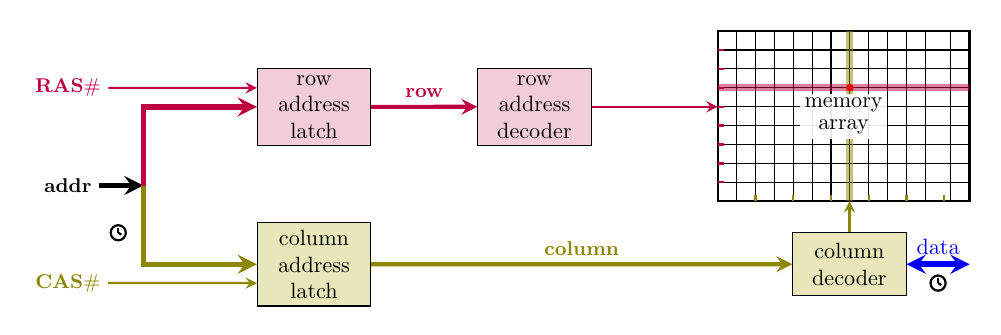
\begin{tikzpicture}[scale=0.8, transform shape,
    block/.style={draw, minimum width=1.8cm, minimum height=1cm, align=center},
    decoder/.style={draw, minimum width=1.8cm, minimum height=1.2cm, align=center},
    signal/.style={->, >=stealth, thick},
    label/.style={font=\small\bfseries}
]

% Origin point - move this to shift entire diagram
\coordinate (origin) at (0,25);

% Row Address Latch - positioned relative to origin
\node[block, text width=1.5cm, fill=purple!20] (rowlatch) at (origin) {row address latch};

% Column Address Latch - positioned relative to row latch
\node[block, text width=1.5cm, fill=olive!20] (collatch) at ([yshift=-2.5cm]rowlatch) {column address latch};

% Row Address decoder - positioned relative to row latch
\node[decoder, text width=1.5cm, fill=purple!20] (rowdecoder) at ([xshift=3.5cm]rowlatch) {row address decoder};

% Column decoder - positioned relative to column latch
\node[block, text width=1.5cm, fill=olive!20] (coldecoder) at ([xshift=8.5cm]collatch) {column decoder};

% Memory array - positioned relative to decoders
\coordinate (array_corner) at ([xshift=2cm, yshift=1.2cm]rowdecoder.east);
\draw[thick] (array_corner) rectangle ([xshift=4cm, yshift=-2.7cm]array_corner);
\foreach \x in {0.3,0.6,0.9,1.2,1.5,1.8,2.1,2.4,2.7,3,3.3,3.7} {
    \draw ([xshift=\x cm]array_corner) -- ([xshift=\x cm, yshift=-2.7cm]array_corner);
}
\foreach \y in {-0.3,-0.6,-0.9,-1.2,-1.5,-1.8,-2.1,-2.4} {
    \draw ([yshift=\y cm]array_corner) -- ([xshift=4cm, yshift=\y cm]array_corner);
}

% Input signals - positioned relative to latches
\node[label, purple] (ras) at ([xshift=-3cm, yshift=0.3cm]rowlatch.west) {RAS$\#$};
\draw[signal, purple] (ras) -- (ras -| rowlatch.west);

\node[label, olive] (cas) at ([xshift=-3cm, yshift=-0.3cm]collatch.west) {CAS$\#$};
\draw[signal, olive] (cas) -- (cas -| collatch.west);

% Address in the middle between the two latches
\node[label] (addr) at ($(rowlatch.west)!0.5!(collatch.west) + (-3,0)$) {addr};
\coordinate (addr_split) at ($(rowlatch.west)!0.5!(collatch.west) + (-1.8,0)$);

\draw[signal, line width=2pt] (addr.east) -- (addr_split);
% Branch to row and column latches
\draw[signal, purple, line width=2pt] (addr_split) -- (addr_split |- rowlatch.west) -- (rowlatch.west);
\draw[signal, olive, line width=2pt] (addr_split) -- (addr_split |- collatch.west) -- (collatch.west);

% Clock symbol relative to addr_split
\drawclock{$(addr_split) + (-0.4,-0.75)$}

% Connections between blocks
\draw[signal, purple, line width=1.5pt] (rowlatch.east) -- node[above, font=\small\bfseries, purple] {row} (rowdecoder.west);
\draw[signal, olive, line width=1.5pt] (collatch.east) -- node[above, font=\small\bfseries, olive] {column} (coldecoder.west);

% Row decoder to memory array with highlighted row
\draw[signal, purple] (rowdecoder.east) -- (rowdecoder.east -| array_corner);
% Draw wordlines and highlight one
\foreach \y in {-0.3,-0.6,-0.9,-1.2,-1.5,-1.8,-2.1,-2.4} {
    \draw[purple, thick] ([yshift=\y cm]array_corner) -- ++(0.1,0);
}
% Highlight one row
\draw[purple, line width=2.5pt, opacity=0.5] ([yshift=-0.9cm]array_corner) -- ([xshift=4cm, yshift=-0.9cm]array_corner);

% Column decoder to memory array with highlighted column
\coordinate (array_bottom) at ([yshift=-2.7cm]array_corner);
\draw[signal, olive] (coldecoder.north) -- (coldecoder.north |- array_bottom);
% Draw bitlines and highlight one
\foreach \x in {0.6,1.2,1.8,2.4,3,3.6} {
    \draw[olive, thick] ([xshift=\x cm, yshift=-2.7cm]array_corner) -- ++(0,0.1);
}
% Highlight one column
\draw[olive, line width=2.5pt, opacity=0.5] ([xshift=2.1cm]array_corner) -- ([xshift=2.1cm, yshift=-2.7cm]array_corner);

% Mark intersection
\fill[red] ([xshift=2.1cm, yshift=-0.9cm]array_corner) circle (0.06);

% Data I/O - horizontal arrow
\draw[signal, blue, line width=2pt, <->] 
  (coldecoder.east) 
    -- node[midway, above, blue]{data} 
  ++(1,0);

% Clock symbol near data - relative to coldecoder
\drawclock{$(coldecoder.east) + (0.5,-0.3)$}

\node[
  align=center, 
  fill=white, 
  fill opacity=0.9,   % background 50% transparent
  text opacity=1,     % text fully visible
  inner sep=2pt
] at ([xshift=2cm, yshift=-1.35cm]array_corner) {memory\\[-2]array};

\end{tikzpicture}
\end{center}

\vspace{-0.2cm}
\textbf{DRAM access sequence:}
\begin{enumerate}
\item Row address on bus → Assert RAS$\#$ to latch row
\item Column address on bus → Assert CAS$\#$ to latch column (after t$_{RCD}$ delay)
\item Data available after CAS latency (CL)
\end{enumerate}

\end{frame}

% Slide: Page Mode DRAM
\begin{frame}{Page Mode DRAM}
\textbf{Allows multiple accesses to different columns within the same row}
\begin{itemize}
\item Saves RAS, RAS to CAS delay, and Row pre-charge
\end{itemize}

\vspace{-0.1cm}
\begin{center}
\begin{tikztimingtable}[
  timing/slope=0.2,
  timing/coldist=0.8cm,
  xscale=1.15,
  timing/rowdist=0.65cm,
  timing/name/.style={font=\small}
]
  RAS\# & 2H L 9L 6H 12.5L \\
  CAS\# & 5H L 2H L 2H L H 8H L 2H L 2H L 2.5H \\
  Addr  & U 1.5D{Row} 1.5U 1.5D{\colorbox{blue!30}{Col}} 1.5U 1.5D{\colorbox{red!30}{Col}} 1.5U 1.5D{\colorbox{orange!30}{Col}} 6U 1.5D{Row} 1.5U 1.5D{\colorbox{green!30}{Col}} 1.5U 1.5D{\colorbox{purple!30}{Col}} 1.5U 1.5D{\colorbox{cyan!30}{Col}} 2.5U \\
  Data  & 6U 2D{\colorbox{blue!30}{Data}} U 2D{\colorbox{red!30}{Data}} U 2D{\colorbox{orange!30}{Data}} 8.5U 2D{\colorbox{green!30}{Data}} U 2D{\colorbox{purple!30}{Data}} U 2D{\colorbox{cyan!30}{Data}} \\
  \extracode
    % Timing annotations
    \begin{scope}[>=stealth]
      %\draw[<->] (0.8,3.6) -- node[above,font=\scriptsize] {tRCD} (2.4,3.6);
      %\draw[<->] (5.6,3.6) -- node[above,font=\scriptsize] {tRP} (10.4,3.6);

      % CL
      \draw[dashed] (4.1,-7.5) -- node[below,font=\scriptsize] {} (4.1,-4);
      \draw[dashed] (6,-7.5) -- node[below,font=\scriptsize] {} (6.1,-5.5);
      \draw[<->] (4.1,-7.5) -- node[below,font=\scriptsize] {CL} (6.1,-7.5);

      % tRCD
      \draw[<->] (2.1,1.5) -- node[above,font=\scriptsize] {tRCD} (5,1.5);
      \draw[dashed] (2.1,1.5) -- node[below,font=\scriptsize] {} (2.1,0.5);
      \draw[dashed] (5,1.5) -- node[below,font=\scriptsize] {} (5,-1.5);
      
      % tRP
      \draw[<->] (12.1,1.5) -- node[above,font=\scriptsize] {tRP} (18,1.5);
      \draw[dashed] (12.1,1.5) -- node[below,font=\scriptsize] {} (12.1,0.5);
      \draw[dashed] (18.1,1.5) -- node[below,font=\scriptsize] {} (18.1,0.5);
    \end{scope}
\end{tikztimingtable}
\end{center}

\vspace{-0.4cm}
\begin{itemize}
\item \textbf{$t_{RP}$}: Row pre-charge time (close current row, open new row)
\item \textbf{CL}: CAS latency (time from CAS to data available)
\item \textbf{Not true random access}: same-row access $\gg$ faster than different-row
\end{itemize}
\end{frame}

% Slide: Synchronous DRAM - SDRAM
\begin{frame}{Synchronous DRAM -- SDRAM}
\textbf{Clock-synchronized (100-200MHz)}
\begin{itemize}
\item All signals referenced to external clock; synchronizes with CPU timing
\end{itemize}

\vspace{0.15cm}
\textbf{4 banks -- multiple rows open simultaneously}
\begin{itemize}
\item One open row per bank; fast column access within 4 open rows
\item ACTIVE to new bank can be issued while accessing current bank
\end{itemize}

\vspace{0.15cm}
\textbf{Command-driven operation}
\begin{itemize}
\item ACTIVE: select bank + row
\item READ/WRITE: select column
\end{itemize}

\vspace{0.15cm}
\textbf{Burst-oriented access}
\begin{itemize}
\item Successive columns in same row; programmable length: 1, 2, 4, 8, full-page
\end{itemize}
\end{frame}

% Slide: SDRAM Features (continued)
\begin{frame}{SDRAM Features (continued)}
\textbf{Programmable Mode Register}
\begin{itemize}
\item CAS latency, burst length, burst type
\end{itemize}

\vspace{0.25cm}
\textbf{Auto pre-charge}: close row at last read/write in burst

\vspace{0.25cm}
\textbf{Auto refresh}: DRAM capacitors leak $\rightarrow$ periodic refresh needed
\begin{itemize}
\item Internal counters automatically generate refresh addresses
\end{itemize}

\vspace{0.3cm}
\begin{block}{Key Advantage}
Bank interleaving: while accessing one bank, another prepares its row $\rightarrow$ higher throughput
\end{block}
\end{frame}

% Slide: SDRAM Timing
\begin{frame}{SDRAM Timing}
\vspace{-0.2cm}
\begin{center}
\begin{tikztimingtable}[
  timing/slope=0.15,
  timing/coldist=0.35cm,
  xscale=1.7,
  timing/rowdist=0.6cm,
  timing/name/.style={font=\small}
]
  clock & L H L H L H L H L H L H L H L H L H L H L H L H L H \\
  cmd   & 2D{\textcolor{cyan}{ACT}} 2U 2D{\textcolor{cyan}{RD}} 2D{\textcolor{cyan}{RD+PC}} 2D{\textcolor{blue}{ACT}} 2U 2D{\textcolor{blue}{RD}} 2D{\textcolor{cyan}{ACT}} 2U 2D{\textcolor{cyan}{RD}} 2D{\textcolor{blue}{RD}} 4U \\
  \\
  Bank  & 2D{\textcolor{cyan}{Bank 0}} 2U 2D{\textcolor{cyan}{Bank 0}} 2D{\textcolor{cyan}{Bank 0}} 2D{\textcolor{blue}{Bank 1}} 2U 2D{\textcolor{blue}{Bank 1}} 2D{\textcolor{cyan}{Bank 0}} 2U 2D{\textcolor{cyan}{Bank 0}} 2D{\textcolor{blue}{Bank 1}} 4U \\
  Addr  & 2D{\textcolor{cyan}{Row i}} 2U 2D{\textcolor{cyan}{Col j }} 2D{\textcolor{cyan}{Col k }} 2D{\textcolor{blue}{Row m}} 2U 2D{\textcolor{blue}{Col n}} 2D{\textcolor{cyan}{Col l}} 2U 2D{\textcolor{cyan}{Col q}} 2D{\textcolor{blue}{Col n+1}} 4U \\
  \\
  Data  & 8U 2D{\textcolor{cyan!50}{Data j}} 2D{\textcolor{cyan!50}{Data k}} 4U 2D{\textcolor{blue}{Data n}} 4U 2D{\textcolor{cyan}{Data q}} 2D{\textcolor{blue}{Data n+1}} \\
  \extracode
    % Vertical grid lines
    \begin{scope}[gray!30, thin]
      \foreach \x in {0,2,...,24} {
        \draw[dashed] (\x+0.15,0.5) -- (\x+0.15,-12);
      }
    \end{scope}
    % Timing annotations
    \begin{scope}[>=stealth, font=\scriptsize]
      % tRCD
      \draw[<->,thick] (5.15,-3) -- node[midway, fill=white, inner sep=1pt]  {$t_{RCD}>$20ns} (1.15,-3);
      \draw (5.15,-2) -- (5.15,-3);
      \draw (1.15,-2) -- (1.15,-4);
      % tRC
     \draw[<->,thick] (1.15,-4) -- node[midway, fill=white, inner sep=1pt] {$_{RC}>$70ns} (15.15,-4);
      \draw (15.15,-2) -- (15.15,-4);
      % tRRD
      \draw[<->,thick] (9.15,-3) -- node[midway, fill=white, inner sep=1pt] {$t_{RRD}>$20ns} (15.15,-3);
      \draw (9.15,-2) -- (9.15,-3);
      % CL
      \draw[<->,thick] (9.15,-9.5) -- node[midway, fill=white, inner sep=1pt] {CL=2} (5.15,-9.5);
      \draw (5.15,-10) -- (5.15,-8);
      \draw (9.15,-9) -- (9.15,-11);

    \end{scope}
\end{tikztimingtable}
\end{center}

\vspace{-0.3cm}
\textbf{Key timing parameters:}
\begin{itemize}
\small
\item $\mathbf{t_{\text{RCD}}}$: Min time from ACTIVE to READ/WRITE command = $\ceil*{\frac{t_{\text{RCD}}(\text{MIN})}{\text{clock period}}}$
\item $\mathbf{t_{\text{RC}}}$: Min time between successive ACTIVE commands to different rows in same bank
\item $\mathbf{t_{\text{RRD}}}$: Min time between successive ACTIVE commands to different banks
\end{itemize}
\end{frame}


\hide{
% Slide: DDR2
\begin{frame}{DDR2}
\textbf{DDR2 doubles bandwidth with 4-bit prefetch}

\vspace{0.2cm}
\begin{columns}[T]
\column{0.48\textwidth}
\textbf{Key improvements:}
\begin{itemize}
\item \textbf{4-bit prefetch}: internally read/write 4$\times$ external bus width
\item DDR2-533 cell works at same frequency as DDR266 or PC133
\item Prefetching increases latency (trade-off)
\item \textbf{Smaller page}: 1KB vs. 2KB
  \begin{itemize}
  \item Reduces activation power
  \end{itemize}
\item \textbf{8 banks} in 1Gb+ densities
  \begin{itemize}
  \item Increases random access performance
  \end{itemize}
\end{itemize}

\column{0.48\textwidth}
\textbf{Power improvements:}
\begin{itemize}
\item 1.8V (vs 2.5V in DDR)
\item Significantly lower power
\end{itemize}

\vspace{0.3cm}
\textbf{Dual channel mode support}

\vspace{0.3cm}
\begin{center}
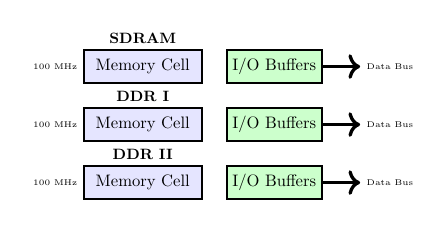
\begin{tikzpicture}[
  scale=0.6,
  transform shape,
  mem cell/.style={draw, thick, minimum width=2.5cm, minimum height=0.7cm, fill=blue!10},
  io buffer/.style={draw, thick, minimum width=1.8cm, minimum height=0.7cm, fill=green!20},
  freq label/.style={font=\tiny, left},
  title label/.style={font=\small, above}
]
  % SDRAM
  \node[mem cell] (sdram mem) at (0,0) {Memory Cell};
  \node[io buffer, right=0.5cm of sdram mem] (sdram io) {I/O Buffers};
  \draw[->, very thick] (sdram io.east) -- ++(0.8,0) node[right, font=\tiny] {Data Bus};
  \node[freq label] at (sdram mem.west) {100 MHz};
  \node[title label] at (sdram mem.north) {\textbf{SDRAM}};

  % DDR I
  \node[mem cell, below=0.5cm of sdram mem] (ddr1 mem) {Memory Cell};
  \node[io buffer, right=0.5cm of ddr1 mem] (ddr1 io) {I/O Buffers};
  \draw[->, very thick] (ddr1 io.east) -- ++(0.8,0) node[right, font=\tiny] {Data Bus};
  \node[freq label] at (ddr1 mem.west) {100 MHz};
  \node[title label] at (ddr1 mem.north) {\textbf{DDR I}};

  % DDR II
  \node[mem cell, below=0.5cm of ddr1 mem] (ddr2 mem) {Memory Cell};
  \node[io buffer, right=0.5cm of ddr2 mem] (ddr2 io) {I/O Buffers};
  \draw[->, very thick] (ddr2 io.east) -- ++(0.8,0) node[right, font=\tiny] {Data Bus};
  \node[freq label] at (ddr2 mem.west) {100 MHz};
  \node[title label] at (ddr2 mem.north) {\textbf{DDR II}};
\end{tikzpicture}
565478\end{center}
\end{columns}
\end{frame}
}

% Slide: DDR Comparison
\begin{frame}{DDR Comparison}
\vspace{-0.2cm}
\begin{center}
\scriptsize
\begin{tabular}{|l|c|c|c|c|c|c|c|}
\hline
& \textbf{Trend} & \textbf{SDRAM} & \textbf{DDR} & \textbf{DDR2} & \textbf{DDR3} & \textbf{DDR4} & \textbf{DDR5} \\
\hline
\textbf{Prefetch depth} & \textcolor{green!60!black}{$\uparrow$} & 1-Bit & 2-Bit & 4-Bit & 8-Bit & Per Bank & 16-Bit \\
\hline
\textbf{Internal clock (MHz)} & $\sim$ & 100-166 & 133-200 & 133-200 & 133-200 & 133-200 & - \\
\hline
\textbf{Data Rate (MT/s)} & \textcolor{green!60!black}{$\uparrow$} & 100-166 & 266-400 & 533-800 & 1066-1600 & 2133-5100 & 3200-6400 \\
\hline
\textbf{Transfer Rate (GB/s)} & \textcolor{green!60!black}{$\uparrow$} & 0.8-1.3 & 2.1-3.2 & 4.2-6.4 & 8.5-14.9 & 17-25.6 & 38.4-51.2 \\
\hline
\textbf{Internal banks} & \textcolor{green!60!black}{$\uparrow$} & 4 & 4 & 4/8 & 8 & 16 & 32 \\
\hline
\textbf{Voltage (V)} & \textcolor{green!60!black}{$\downarrow$} & 3.3 & 2.5-2.6 & 1.8 & 1.35-1.5 & 1.2 & 1.1 \\
\hline
\textbf{CAS Latency (cycles)} & \textcolor{red}{$\uparrow$} & 2-3 & 2-3 & 3-5 & 5-11 & 12-18 & 32-40 \\
\hline
\textbf{Actual Latency (ns)} & $\sim$ & $\sim$10 & $\sim$10 & $\sim$10 & $\sim$11 & $\sim$10 & $\sim$12 \\
\hline
\textbf{Max DIMM size (GB)} & \textcolor{green!60!black}{$\uparrow$} & - & 1 & 4 & 16 & 64 & 256 \\
\hline
\end{tabular}
\end{center}

\vspace{0.1cm}
\textbf{Key trends:}
\begin{itemize}
\item \textcolor{green!60!black}{Bandwidth doubles each generation} (prefetch depth $\uparrow$, internal clock $\sim$)
\item \textcolor{green!60!black}{Power efficiency improves} (voltage $\downarrow$)
\item \textcolor{green!60!black}{More banks} = better parallelism for multiple requests
\item \textcolor{red}{CAS latency $\uparrow$ in cycles}, but \textcolor{blue}{stays $\sim$10-12ns} (clocks compensate)
\end{itemize}
\end{frame}

% Slide: ECC Memory
\begin{frame}{ECC: Error Correcting Code Memory}
\textbf{What does ECC do?}
\begin{itemize}
\item \textbf{SECDED:} Single Error Correction, Double Error Detection
\item Uses 8 extra bits for every 64 data bits (72-bit total)
\item \textcolor{green!60!black}{Corrects:} 1-bit errors (automatically, transparent)
\item \textcolor{blue}{Detects:} 2-bit errors (reports error, cannot correct)
\item \textbf{Implementation:} Memory controller generates/checks ECC; DIMM stores it
\item \textbf{DDR5 on-die ECC:} Additional protection inside DRAM chips (separate)
\end{itemize}

\vspace{0.3cm}
\textbf{Why is ECC needed?}
\begin{itemize}
\item DRAM cells can experience bit flips due to:
  \begin{itemize}
  \item Cosmic rays, alpha particles (from packaging)
  \item Electrical noise, voltage fluctuations
  \item Cell leakage, manufacturing defects
  \end{itemize}
\item \textbf{Error rates} (Google study, 2009):
  \begin{itemize}
  \item \textcolor{green!60!black}{Correctable errors (soft):} $\sim$32\% of servers per year
  \item \textcolor{red}{Uncorrectable errors (hard):} $\sim$1.3\% of servers per year
  \item Average: 2000-6000 correctable errors per GB per year
  \end{itemize}
\end{itemize}
\end{frame}

% Slide: DIMM
\begin{frame}{DIMM: Dual In-line Memory Module}
\textbf{A small circuit board that holds memory chips}

\vspace{0.2cm}
\begin{columns}[T]
\column{0.6\textwidth}
\textbf{Physical:}
\begin{itemize}
\item DDR4/DDR5: 288 pins
\item Single/dual-sided configurations
\end{itemize}

\vspace{0.15cm}
\textbf{Data path:}
\begin{itemize}
\item 64-bit wide (non-ECC)
\item 72 bits with ECC
\item DDR: both clock edges
\item $\Rightarrow$ 128 bits/clock
\end{itemize}

\column{0.3\textwidth}
\begin{center}
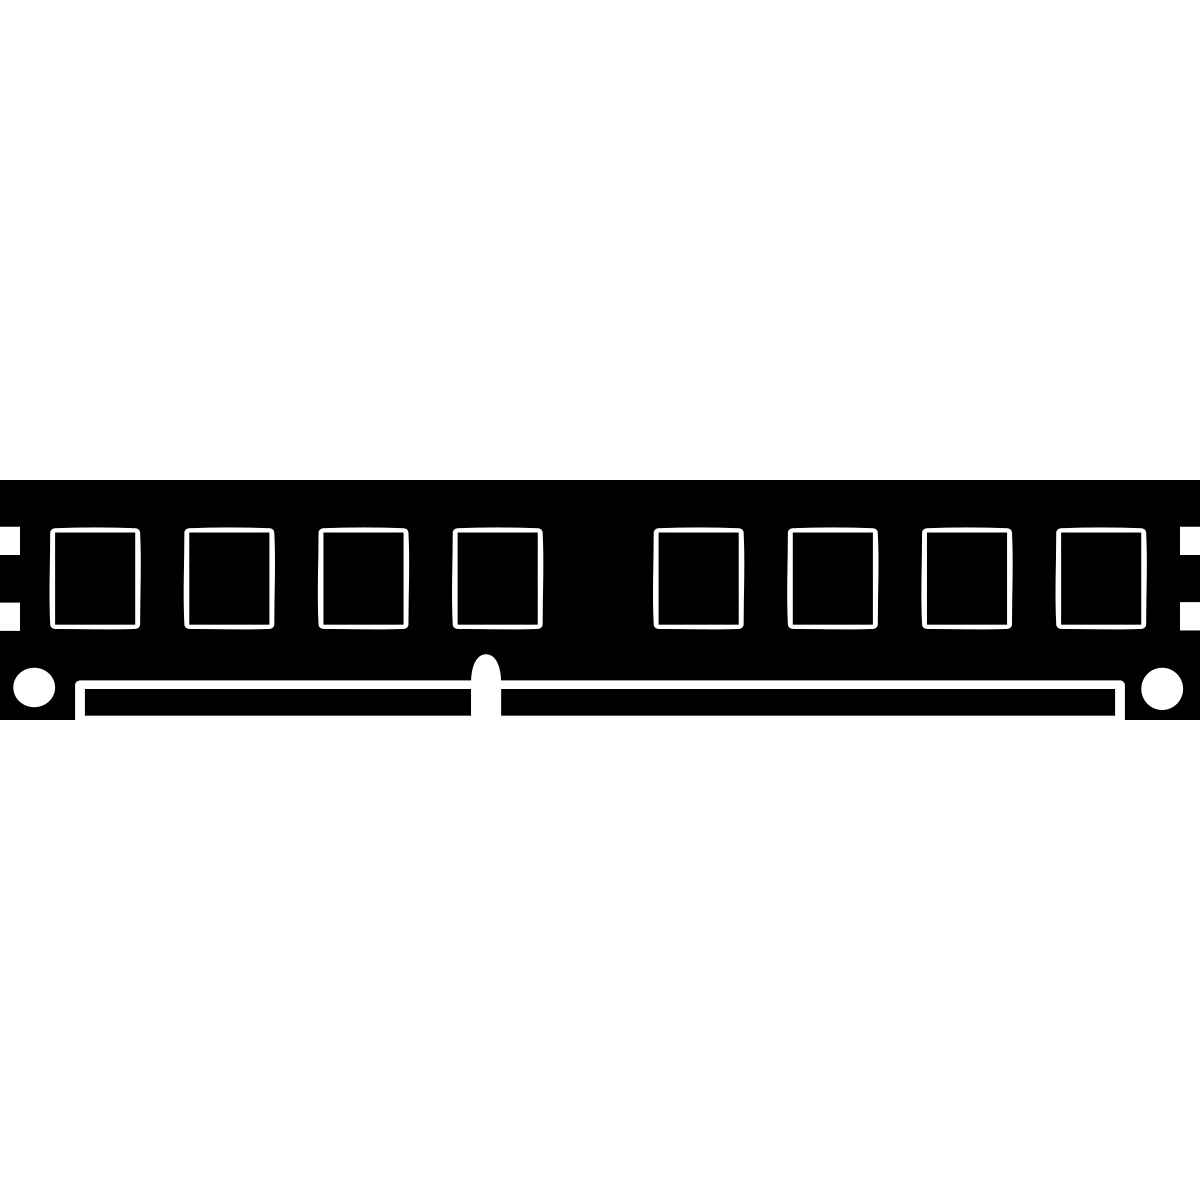
\includegraphics[width=0.6\textwidth,angle=90,width=\textwidth,keepaspectratio]{figures/noun-ram-2198352.pdf}
\end{center}
\end{columns}
\end{frame}

% Slide: DRAM Controller
\begin{frame}{DRAM Controller}
\textbf{What the DRAM controller does:}

\vspace{0.3cm}
\begin{itemize}
\item \textbf{Address translation:}
  \begin{itemize}
  \item Splits memory address into Row and Column addresses
  \item Routes to correct bank and chip
  \end{itemize}

\vspace{0.2cm}
\item \textbf{Timing control:}
  \begin{itemize}
  \item Generates RAS\# (Row Address Strobe) and CAS\# (Column Address Strobe) signals
  \item Enforces timing constraints ($t_{\text{RCD}}$, $t_{\text{RC}}$, $t_{\text{RRD}}$, etc.)
  \end{itemize}

\vspace{0.2cm}
\item \textbf{Refresh management:}
  \begin{itemize}
  \item DRAM cells lose charge over time ($\sim$64ms)
  \item Controller periodically refreshes all rows
  \item Refresh operations steal bandwidth from normal accesses
  \end{itemize}

\vspace{0.2cm}
\item \textbf{Command scheduling:}
  \begin{itemize}
  \item Out-of-order execution to maximize bandwidth
  \item Row buffer hit optimization (keep frequently-used rows open)
  \end{itemize}
\end{itemize}
\end{frame}

% Slide: DRAM Controller Architecture
\begin{frame}{DRAM Controller Architecture}
\begin{center}
\begin{circuitikz}[
  transform shape,
  unit/.style={muxdemux, external pins width=0, align=center, font=\small},
  textnode/.style={above, font=\footnotesize, align=center}
]
  % Address decoder
  \node[unit, muxdemux def={Lh=3, Rh=3, w=3.5, NL=1, NR=1}]
    (decoder) at (0,0) {Address\\Decoder};

  % Time delay generator
  \node[unit, muxdemux def={Lh=3, Rh=3, w=3.5, NL=1, NB=1, NR=2},
     right=1.8cm of decoder] (timegen) {Time\\Delay\\Generator};

  % Address mux (using circuitikz mux)
  \node[unit, muxdemux def={Lh=3, Rh=1.5, w=2.5, NL=2, NT=1, NR=1},
        below=5mm of decoder] (addrmux) {Addr\\Mux};

  % DRAM chip
  \node[unit, muxdemux def={Lh=3, Rh=3, w=3.5, NL=4, NR=1},
        fill=blue!10, anchor=lpin 3] at ([xshift=1.8cm]addrmux.rpin 1 -| timegen.east) (dram) {DRAM};

  \coordinate (input) at ([xshift=-3.5cm, yshift=-1cm]decoder.west);
  \coordinate (rw) at ([yshift=-3mm]input |- addrmux.south);

  % Address bus inputs
  \draw[->, thick] (input) -- ++(0.5,0) |- node[textnode, near end] {A[20:23] (\textcolor{red}{Chip})} (decoder.lpin 1);
  \draw[->, thick] ([xshift=5mm]input) |- node[textnode, near end] {A[10:19] (\textcolor{green}{Row})} (addrmux.lpin 1);
  \draw[->, thick] ([xshift=5mm]input) |- node[textnode, near end] {A[0:9] (\textcolor{blue}{Col})} (addrmux.lpin 2);

  % Decoder to Time delay gen (Chip select)
  \draw[->, thick] (decoder.rpin 1) -- node[textnode] {\textcolor{red}{Chip}\\\textcolor{red}{Select}} (timegen.lpin 1);

  % Time delay gen to DRAM (RAS# and CAS#)
  \draw[->, thick] (timegen.rpin 1) -- node[textnode] {\textcolor{green}{RAS\#}}  ++(1.4, 0) |- 
    (dram.lpin 1);
  \draw[->, thick] (timegen.rpin 2) -- node[textnode] {\textcolor{blue}{CAS\#}}  ++(1, 0) |-
    (dram.lpin 2);

  % Time delay gen to Address mux select
  \draw[->, thick] (timegen.bpin 1) -- ++(0, -0.3) -| node[textnode, pos=0.3] {Select} (addrmux.tpin 1);

  % Address mux to DRAM (Memory address bus)
  \draw[->, thick] (addrmux.rpin 1) -- node[textnode] {Memory Addr Bus} (dram.lpin 3);

  % R/W# signal
  \draw[->, thick] (rw) -| node[textnode, pos=0.1] {R/W\#} ([xshift=-5mm]dram.lpin 4) -- (dram.lpin 4);

  % Data output
  \draw[->, thick] (dram.rpin 1) -- node[textnode] {D[0:7]} ([xshift=1.5cm]dram.rpin 1);

\end{circuitikz}
\end{center}

\vspace{0.2cm}
\textbf{Key components:}
\begin{itemize}
\item Address decoder selects chip based on high address bits
\item Time delay generator creates properly-timed RAS\# and CAS\# signals
\item Address mux switches between Row (A[10:19]) and Column (A[0:9]) addresses
\end{itemize}
\end{frame}

% Slide: DRAM Controller Channels
\begin{frame}{DRAM Controller: Dual-Channel Architecture}
\textbf{Modern controllers support multiple independent channels:}

\vspace{0.3cm}
\begin{columns}[T]
\column{0.58\textwidth}
\textbf{Each channel operates independently:}
\begin{itemize}
\item Separate command/address/data buses
\item Independent scheduling and buffering
\item Write buffer: 32 cache lines per channel
\item Throughput: 8 bytes/cycle per channel
\end{itemize}

\vspace{0.3cm}
\textbf{Address distribution:}
\begin{itemize}
\item Hash function spreads addresses across channels
\item Balances load for maximum bandwidth
\item Reduces hotspot contention
\end{itemize}

\column{0.38\textwidth}
\vspace{0.2cm}
\textbf{Best practices:}
\begin{itemize}
\item Populate both channels equally
\item Use matched DIMMs (same speed/capacity)
\item More DIMMs = more open pages:
  \begin{itemize}
  \item Each DIMM: 4-8 banks
  \item $n$ DIMMs = $4n$ to $8n$ open pages
  \item Better random access performance
  \end{itemize}
\end{itemize}

\vspace{0.3cm}
\textbf{Why it matters:}\\
Unbalanced channels waste half your bandwidth!
\end{columns}
\end{frame}


% Slide: DRAM Scheduling Policies
\begin{frame}{DRAM Scheduling Policies}
\textbf{Scheduling policy:} determines order in which requests are serviced

\vspace{0.4cm}
\textbf{Prioritization considerations:}
\begin{itemize}
\item Request age (oldest first)
\item Row buffer hit/miss status (hits first)
\item Request type (read vs write)
\item Request criticality (will it stall the processor?)
\item Interference to other cores
\end{itemize}

\vspace{0.4cm}
\textbf{Example: FR-FCFS} (first ready, first come first served)
\begin{enumerate}
\item Prioritize row-buffer hits
\item Then prioritize older requests
\item[] \textcolor{green!60!black}{FR-FCFS maximizes throughput} but \textcolor{red}{can starve requests $\rightarrow$ unfairness, high tail latency}
\end{enumerate}
\end{frame}

% Slide: Row Buffer Management Policies
\begin{frame}{Row Buffer Management Policies}
\textbf{Open row} -- keep the row open after an access
\begin{itemize}
\item \textcolor{green!60!black}{Row hit if same row accessed again}
\item \textcolor{red}{Row conflict + wasted energy if different row}
\end{itemize}

\vspace{0.4cm}
\textbf{Closed row} -- close after access (if no pending requests need same row)
\begin{itemize}
\item \textcolor{green!60!black}{Avoids conflict if different row accessed}
\item \textcolor{red}{Extra activate latency if same row accessed again}
\end{itemize}

\vspace{0.4cm}
\textbf{Adaptive} -- predict whether next access will be to same row
\end{frame}

\begin{frame}{High Bandwidth Memory Package}
% Define colors for mixing
\colorlet{basecolor}{cyan!70}
\colorlet{emibcolor}{blue!50!cyan}

% Text overlay at top right
\begin{tikzpicture}[remember picture, overlay]
\node[anchor=north east, fill=white, fill opacity=0.9, text opacity=1,
      draw=blue!50, line width=0.5pt, rounded corners=3pt, inner sep=5pt, text width=5cm, font=\small]
  at ([xshift=-8mm, yshift=-18mm]current page.north east) {
\only<1>{
\textbf{Package Overview}
\begin{itemize}\setlength\itemsep{0.1em}
\item Circuit board with substrate
\item Interconnect infrastructure
\end{itemize}
}
\only<2>{
\textbf{HBM Stack (3D DRAM)}
\begin{itemize}\setlength\itemsep{0.1em}
\item Multiple DRAM dies stacked vertically
\item Connected via \textbf{TSVs} (Through-Silicon Vias)
\item TSVs enable high-density 3D integration
\end{itemize}
}
\only<3>{
\textbf{Base Die \& Logic}
\begin{itemize}\setlength\itemsep{0.1em}
\item Base die interfaces with HBM stack
\item Contains memory controllers
\item Very wide bus (1024+ bits)
\end{itemize}
}
\only<4>{
\textbf{EMIB Integration}
\begin{itemize}\setlength\itemsep{0.1em}
\item \textbf{EMIB:} Embedded Multi-die Interconnect Bridge
\item High-density die-to-die connections
\item Connects compute dies to memory
\item Short signal paths, high bandwidth
\end{itemize}
}
};
\end{tikzpicture}

% Illustration at bottom
\vfill
\begin{tikzpicture}[scale=0.7, every node/.style={scale=0.7},
    >=Stealth,
    thick,
    circuit/.style={rectangle, fill=green!60!black, draw=green!40!black, text=white, font=\tiny},
    substrate/.style={rectangle, fill=cyan!60, draw=cyan!80!black, text=white, font=\tiny},
    hbm/.style={rectangle, fill=red!70!brown, draw=brown!50!black, text=white, font=\tiny, align=left},
    base/.style={rectangle, fill=basecolor, draw=cyan!80!black, text=white, font=\tiny, align=left},
    phy/.style={rectangle, fill=emibcolor, draw=blue!70!black, text=white, font=\tiny},
    emib/.style={rectangle, fill=emibcolor, draw=blue!70!black, text=white, font=\tiny},
    compute/.style={rectangle, fill=blue!60!red!40, draw=blue!80!red!60, text=white, font=\tiny},
    tsv/.style={rectangle, fill=yellow, draw=black, minimum size=2mm, inner sep=0pt},
    ball/.style={circle, fill=gray!60, draw=black!80, minimum size=3mm, inner sep=0pt},
    bump/.style={ball, fill=gray!60, draw=black!80, minimum size=1mm},
    ubump/.style={bump, fill=gray!60, draw=black!80, minimum size=0.5mm},
    graybump/.style={circle, fill=gray!60, draw=black!80, inner sep=0pt, anchor=south},
    label/.style={font=\tiny},
    small label/.style={font=\scriptsize}
  ]

% Package Substrate (base layer)
\node[substrate, minimum width=10cm, minimum height=1.3cm]
  (substrate) at (5.5,0.85) {Package Substrate};

% Package Balls (positioned at bottom of substrate)
\foreach \i in {0,1,...,19} {
  \node[ball, anchor=north] (ball\i) at ([xshift=2mm + \i * 5mm]substrate.south west) {};
}

% Package Bumps (positioned at top of substrate)
\foreach \i in {0,1,...,6} {
  \node[bump, anchor=south] (pbump\i) at ([xshift=2mm + \i * 4mm]substrate.north west) {};
}

% Basic Logic Die Bumps (positioned above substrate)
\foreach \i in {0,1,...,11} {
  \node[bump, anchor=south] (blbump\i) at ([xshift=-2mm - \i * 4mm]substrate.north east) {};
}

% Circuit Board (positioned below balls, relative to ball1)
\node[circuit, minimum width=13.5cm, minimum height=0.7cm, anchor=north]
  (board) at ([xshift=3.5cm]ball1.south) {Circuit Board};

% Standard Package Traces
%\draw[thick, gray!40] (1.8,0.8) -- (1.8,1.3) -- (3.5,1.3) -- (3.5,1.8);
%\draw[thick, gray!40] (2.5,0.8) -- (2.5,1.45) -- (4.5,1.45) -- (4.5,1.8);

% Base Die (positioned relative to substrate)
\node[base, minimum width=3.8cm, minimum height=0.8cm, anchor=south west, text width=3.5cm]
  (basedie) at (pbump0.north -| substrate.west) {Base Die};

% Base Logic Die (positioned relative to Base Die, to its right)
\node[base, fill=basecolor!80, minimum width=5.8cm, minimum height=0.8cm, anchor=west]
  (baselogic) at ([xshift=4mm]basedie.east) {Base Logic Die};

% PHY blocks
\node[phy, fill=emibcolor!70, minimum width=0.7cm, minimum height=0.4cm, anchor=south east]
  (phy0) at ([xshift=-1mm, yshift=1mm]basedie.south east) {PHY};
\node[phy, fill=emibcolor!70, minimum width=0.7cm, minimum height=0.4cm, anchor=south west]
  (phy1) at ([xshift=1mm, yshift=1mm]baselogic.south west) {PHY};

\node[emib, fill=emibcolor!90, minimum width=3.4cm, minimum height=0.4cm, anchor=north west, align=right, text width=3.2cm]
  (emib) at ([xshift=-2mm]phy0.west |- substrate.north) {EMIB};



% HBM Stack (4 dies, positioned relative to Base Die)
\foreach \j in {0,1,...,3} {
  \node[hbm, minimum width=2.7cm, minimum height=0.6cm, anchor=south west, text width=2.5cm]
    (hbm\j) at ([xshift=1mm, yshift=\j * 8mm + 1mm]basedie.north west) {HBM DRAM\\Die};
  % TSVs (yellow bumps, positioned relative to hbm\j.east)
  \foreach \i in {0,1,...,4} {
    \node[tsv, minimum width=0.08cm, minimum height=0.4cm, anchor=north] (tsv\j-\i) at ([xshift=-1mm - \i * 2mm]hbm\j.north east) {};
  }
  % µBumps at bottom of each (positioned south of TSVs)
  \foreach \i in {0,1,...,4} {
    \node[bump, anchor=north] (ubump\j-\i) at (tsv\j-\i.south |- hbm\j.south) {};
    \draw (tsv\j-\i.south) -- (ubump\j-\i.north);
  }
}

% Base Die TSVs and bumps (below HBM µBumps)
\foreach \i in {0,1,...,4} {
  % TSV in Base Die
  \node[tsv, minimum width=0.08cm, minimum height=0.3cm, anchor=north] (basetsv\i) at (ubump0-\i.south) {};
  % Bump at bottom of Base Die TSV
  \node[bump, anchor=north] (basebump0\i) at ([xshift=-2mm * \i]phy0.east |- basedie.south) {};
  % Wiring between HBM bump and Base Die TSV
  \draw[very thin, white] (basetsv\i.south) -- ++(0,-1mm - \i * 0.5mm) -| (basebump0\i.north);
  % Bump at bottom of Base Logic Die TSV
  \node[bump, anchor=north] (baselbump1\i) at ([xshift=2mm * \i]phy1.west |- baselogic.south) {};
  % Wiring between Base Logic Die TSV and Base
  \draw[very thin, white] (basebump0\i.south) -- ++(0,-1mm - \i * 0.5mm) -| (baselbump1\i.north);
}

% EMIB section
%\node[emib, rectangle, minimum width=2.5cm, minimum height=0.55cm, text=white, font=\tiny]
%  (emib) at (5.05,1.775) {EMIB};


% Short Wires in EMIB
%\foreach \x in {4.0,4.3,4.6,4.9,5.2} {
%  \draw[gray!40, very thin] (\x,1.55) -- (\x,1.65);
%}



% F2F µBumps (gray circles above Base Logic Die, using calc)
\foreach \i in {0,1,...,8} {
  \node[graybump, minimum size=0.5mm] (f2fbump0-\i) at ([xshift=-2mm - \i * 3mm]baselogic.north east) {};
  \node[graybump, minimum size=0.5mm] (f2fbump1-\i) at ([xshift=2mm + \i * 3mm]baselogic.north west) {};
  %\node[graybump, minimum size=0.5mm] at ($(baselogic.north west) + (\x,0.06)$) {};
}

% Compute Dies (positioned above F2F µBumps)
\node[compute, minimum width=2.8cm, minimum height=0.55cm, align=center, anchor=south west]
  (compute1) at (f2fbump1-7.north -| baselogic.west) {Compute/FPGA/Mem\\Die};
\node[compute, minimum width=2.8cm, minimum height=0.55cm, align=center, anchor=south east]
  (compute0) at (f2fbump1-7.north -| baselogic.east) {Compute/FPGA/Mem\\Die};

% Interconnect lines
%\draw[gray!40] (5.0,2.2) -- (5.0,2.45) -- (8.5,2.45) -- (8.5,2.7);
%\draw[gray!40] (6.0,2.2) -- (6.0,2.55) -- (9.0,2.55) -- (9.0,2.7);

% µBumps between EMIB and dies (positioned relative to base dies)
%\foreach \i in {0,1,...,3} {
%  \node[graybump, minimum size=1mm] (emibump\i) at ([xshift=33mm + \i * 3mm]basedie.north west) {};
%}

% Annotations
%\draw[->, thick] (-1.5,0.6) -- (0.4,0.9);
\node[label, anchor=east] (packagetrace) at ([xshift=-1cm]substrate.west) {\shortstack{Standard\\Package Trace}};
\draw[->, thick] (packagetrace.east) -- (substrate.west);

%\draw[->, thick] (-1.2,1.3) -- (0.5,1.7);
\node[label, anchor=east] (bumpslabel) at ([xshift=-1.5cm]pbump0) {Bumps};
\draw[->, thick] (bumpslabel.east) -- (pbump0.west);

\foreach \i in {0,1,...,3} {
  \draw[very thin] (pbump\i.south) -- ++(0,-1cm) -| (ball\i.north);
  %\draw[->, thick] ([xshift=-5mm]ball\i) -- ([xshift=-\ballRadius cm]ball\i);
}

%\draw[->, thick] ([xshift=-5mm]ball0) -- ([xshift=-\ballRadius cm]ball0);
\node[label, anchor=east, align=center] (packageballs) at ([xshift=-1.5cm,yshift=1mm]ball0) {Package\\Balls};
\draw[->, thick] (packageballs.east) -- (ball0.west);

%\draw[->, thick] (packageballs.east) -- (ball0.west);
\node[label] (tsvlabel) at ([xshift=10mm]tsv3-0.east) {TSV};
\draw[->, thick] (tsvlabel.west) -- (tsv3-0.east);

%\draw[->, thick] (4.3,4.3) -- (3.3,3.7);
%\node[label] (ubumps) at (4.5,4.5) {µBumps};

%\draw[->, thick] (3.0,5.2) -- (4.2,2.75);
%\node[label, anchor=south] (shortwires) at (2.8,5.3) {Short Wires};

%\draw[->, thick] (9.5,3.8) -- (8.0,2.9);
%\node[label] (f2fbumps) at (10,3.8) {\shortstack{F2F\\µBumps}};

%\draw[->, thick] (10.5,2.0) -- (9.5,2.45);

\end{tikzpicture}
\end{frame}

% Slide: HBM Architecture
\begin{frame}{High Bandwidth Memory (HBM)}
\begin{columns}[T]
\column{0.5\textwidth}
\begin{center}
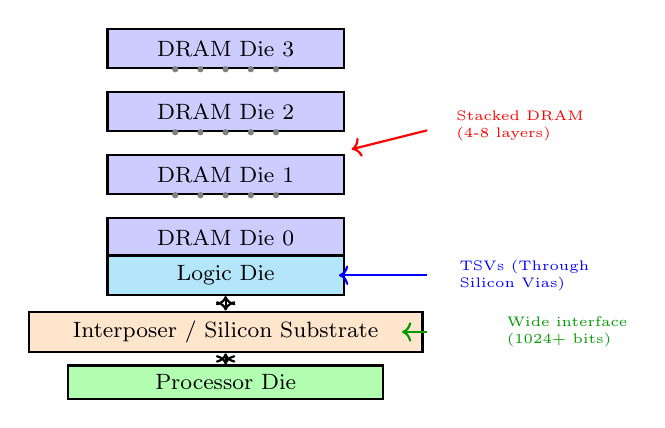
\begin{tikzpicture}[scale=0.8,
    die/.style={draw, thick, fill=blue!20, minimum width=3cm, minimum height=0.5cm, font=\footnotesize},
    substrate/.style={draw, thick, fill=green!30, minimum width=4cm, minimum height=0.4cm, font=\footnotesize},
    tsv/.style={circle, fill=gray, inner sep=0.8pt}
]

% Processor die at bottom
\node[substrate] (proc) at (0,-0.5) {Processor Die};

% Interposer
\node[substrate, minimum width=5cm, fill=orange!20] (interposer) at (0,0.3) {Interposer / Silicon Substrate};

% HBM Stack - using loop
\foreach \i in {0,1,2,3} {
    \node[die, yshift=\i*8mm] (hbm\i) at (0,1.8) {DRAM Die \i};
    % TSVs represented as small circles
    \foreach \x in {-0.8,-0.4,0,0.4,0.8} {
        \node[tsv] at ([xshift=\x cm]hbm\i.south) {};
    }
}

% Base logic die
\node[die, fill=cyan!30] (logic) at (0,1.2) {Logic Die};

% Connections
\draw[thick, <->] (proc.north) -- (interposer.south);
\draw[thick, <->] (interposer.north) -- (logic.south);

% Labels with annotations
\draw[->, thick, red] (3.2,3.5) -- (2,3.2) node[anchor=west, xshift=1.2cm, yshift=0.3cm, align=left, font=\tiny] {Stacked DRAM\\(4-8 layers)};
\draw[->, thick, blue] (3.2,1.2) -- (1.8,1.2) node[anchor=west, xshift=1.4cm, align=left, font=\tiny] {TSVs (Through\\Silicon Vias)};
\draw[->, thick, green!60!black] (3.2,0.3) -- (2.8,0.3) node[anchor=west, xshift=1.2cm, align=left, font=\tiny] {Wide interface\\(1024+ bits)};

\end{tikzpicture}
\end{center}

\column{0.5\textwidth}
\textbf{Key features:}
\begin{itemize}
\item \textbf{3D stacked} DRAM dies
\item Connected via TSVs
\item Very wide bus (1024-4096 bits)
\item Short signal paths
\item Lower voltage/power
\end{itemize}

\vspace{0.3cm}
\textbf{Used in:}
\begin{itemize}
\item GPUs (graphics cards)
\item AI accelerators
\item High-performance computing
\end{itemize}
\end{columns}
\end{frame}

% Slide: HBM vs DDR
\begin{frame}{HBM vs DDR Memory}
\begin{center}
\begin{tabular}{l|c|c}
\textbf{Property} & \textbf{DDR (e.g., DDR5)} & \textbf{HBM (e.g., HBM3)} \\
\hline
\textbf{Architecture} & Planar (2D) & Stacked (3D) \\
\textbf{Bus width} & 64 bits/channel & 1024+ bits/stack \\
\textbf{Bandwidth} & 30-50 GB/s/channel & 300-600 GB/s/stack \\
\textbf{Capacity} & High (32-128GB+) & Lower (8-24GB/stack) \\
\textbf{Power efficiency} & Good & Better \\
\textbf{Cost} & \textcolor{green!60!black}{Low} & \textcolor{red}{High} \\
\textbf{Packaging} & Standard DIMMs & \textcolor{red}{Integrated (not upgradeable)} \\
\end{tabular}
\end{center}

\vspace{0.4cm}
\textbf{Why not always use HBM?}
\begin{itemize}
\item \textcolor{red}{Expensive} -- complex 3D packaging, low yields
\item \textcolor{red}{Limited capacity} -- fewer dies per stack than DIMMs
\item \textcolor{red}{Not upgradeable} -- soldered to package/interposer
\item Only worth it when \textcolor{green!60!black}{bandwidth is critical} (GPUs, AI training)
\end{itemize}
\end{frame}

\section{PCIe Architecture}

% Slide: PCIe Overview
\begin{frame}{PCIe: PCI Express}
\textbf{PCIe is a layered protocol}

\begin{itemize}
\item \textbf{Compatible with the PCI addressing model}
  \begin{itemize}
  \item All existing applications and drivers operate unchanged
  \end{itemize}

\vspace{0.3cm}
\item \textbf{Software layers} generate read and write requests

\vspace{0.3cm}
\item \textbf{Hardware layers} process and transmit data:
  \begin{itemize}
  \item \textcolor{blue}{Transaction Layer}: Splits data to packets
  \item \textcolor{green!60!black}{Data Link Layer}: Ensures data integrity (adds sequence numbers and CRC)
  \item \textcolor{orange}{Physical Layer}: Transmits the packets (connector, voltage levels, etc.)
  \end{itemize}
\end{itemize}

\vspace{0.3cm}
\begin{alertblock}{Key Benefit}
Layered design ensures reliable delivery of packets across the PCIe link
\end{alertblock}
\end{frame}

% Slide: PCIe Layer Architecture with Diagram
\begin{frame}{PCIe Layer Architecture}
\begin{center}
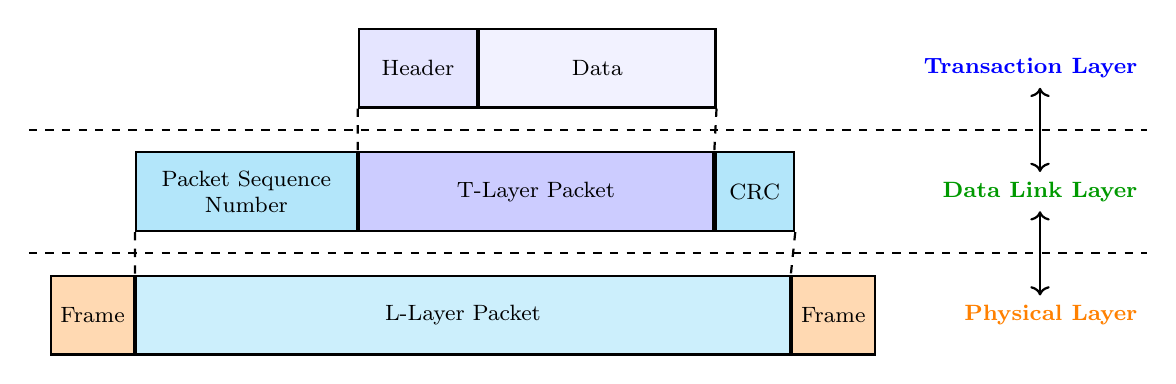
\begin{tikzpicture}[scale=0.9,
    box/.style={draw, thick, minimum height=1cm, align=center, font=\footnotesize},
    layer/.style={draw=none, align=center, font=\footnotesize}
]

% Top level - Original packet
\node[box, fill=blue!10, minimum width=1.5cm] (header) at (0,0) {Header};
\node[box, fill=blue!5, minimum width=3cm, anchor=west] (data) at (header.east) {Data};



% T-Layer Packet - below header, spanning from header.west to data.east
\node[box, fill=blue!20, anchor=north west, minimum width=4.5cm] (tlpacket) at ([yshift=-6mm]header.south west) {T-Layer Packet};

% Dashed lines showing T-Layer includes header and data
\draw[dashed, thick] (header.south west) -- (tlpacket.north west);
\draw[dashed, thick] (data.south east) -- (tlpacket.north east);

% Packet Sequence Number - left of T-Layer Packet, wider and exactly 2 rows
\node[box, fill=cyan!30, minimum width=2.8cm, anchor=east] (pseq) at (tlpacket.west) {Packet Sequence\\Number};

% CRC - right of T-Layer Packet, adjacent
\node[box, fill=cyan!30, minimum width=1cm, anchor=west] (crc1) at (tlpacket.east) {CRC};


% L-Layer Packet - below pseq, spanning from pseq.west to crc1.east
\node[box, fill=cyan!20, minimum width=8.3cm, anchor=north west] (llpacket) at ([yshift=-6mm]pseq.south west) {L-Layer Packet};

% Dashed lines showing L-Layer includes pseq, tlpacket, and crc1
\draw[dashed, thick] (pseq.south west) -- (llpacket.north west);
\draw[dashed, thick] (crc1.south east) -- (llpacket.north east);

% Frame boxes - left and right of L-Layer Packet, touching
\node[box, fill=orange!30, minimum width=1cm, anchor=east] (frame1) at (llpacket.west) {Frame};
\node[box, fill=orange!30, minimum width=1cm, anchor=west] (frame2) at (llpacket.east) {Frame};

% Physical Layer label - positioned similarly
\node[layer, right=of frame2] (physlayer) {\textbf{\textcolor{orange}{Physical Layer}}};
\node[layer, anchor=east] (linklayer) at (crc1 -| physlayer.east) {\textbf{\textcolor{green!60!black}{Data Link Layer}}};
\node[layer, anchor=east] (translayer) at (data -| physlayer.east) {\textbf{\textcolor{blue}{Transaction Layer}}};

% Dashed line separator below
\draw[dashed, thick] ([yshift=-3mm,xshift=-1.5cm]header.south -| pseq.west) -- ([yshift=-3mm]translayer.east |- header.south);
\draw[dashed, thick] ([yshift=-3mm,xshift=-1.5cm]pseq.south west) -- ([yshift=-3mm]linklayer.east |- pseq.south);

% Arrows between layers
\draw[<->, thick] (linklayer.south) -- (physlayer.north -| linklayer);
\draw[<->, thick] (linklayer.north) -- (translayer.south -| linklayer);

\end{tikzpicture}
\end{center}

\vspace{0.3cm}
\footnotesize
Data flows top-to-bottom (TX) and bottom-to-top (RX) through the layers
\end{frame}

% Slide: Physical Layer
\begin{frame}{PCIe Physical Layer}
\textbf{Responsibilities:}
\begin{itemize}
\item \textbf{Transmits packets} received from the Data Link Layer
\item \textbf{Connector definition}: Physical form factor and pinout
\item \textbf{Electrical specifications}: Voltage levels, timing, signaling
\item \textbf{Serialization/Deserialization}: Converts parallel data to serial transmission
\end{itemize}

\vspace{0.3cm}
\textbf{Key Features:}
\begin{itemize}
\item Point-to-point serial links (lanes)
\item Multiple lanes can be aggregated: x1, x4, x8, x16
\item High-speed differential signaling
\item Supports multiple generations (PCIe 4.0: 16 GT/s, PCIe 5.0: 32 GT/s)
\end{itemize}

\vspace{0.3cm}
\begin{alertblock}{Physical Layer Goal}
Reliable transmission of bits across the physical medium
\end{alertblock}
\end{frame}

% Slide: Data Link Layer
\begin{frame}{PCIe Data Link Layer}
\textbf{Responsibilities:}
\begin{itemize}
\item \textbf{Ensure data integrity}: Adds sequence number and CRC to each transaction layer packet
\item \textbf{Credit-based flow control protocol}
\item \textbf{Automatic retry} of corrupted packets detected by CRC checking
\end{itemize}

\vspace{0.3cm}
\textbf{Flow Control:}
\begin{itemize}
\item Packets only transmitted when receiver has buffer space available
\item \textcolor{green!60!black}{Eliminates packet retries due to buffer overflow}
\item \textcolor{green!60!black}{Saves bus bandwidth} (no wasted transmission attempts)
\end{itemize}

\vspace{0.3cm}
\textbf{Error Handling:}
\begin{itemize}
\item CRC checks data integrity
\item NAK (Negative Acknowledgment) triggers automatic retransmission
\item Transparent to upper layers
\end{itemize}
\end{frame}

% Slide: Transaction Layer
\begin{frame}{PCIe Transaction Layer}
\textbf{Responsibilities:}
\begin{itemize}
\item \textbf{Receives} read and write requests from the software layer
\item \textbf{Creates} request packets for transmission to the link layer
\item \textbf{Receives} response packets from the link layer
\item \textbf{Matches} responses with original requests using unique identifiers
\end{itemize}

\vspace{0.3cm}
\textbf{Packet Format Features:}
\begin{itemize}
\item Supports 32-bit and extended 64-bit memory addressing
\item Packet attributes for optimization:
  \begin{itemize}
  \item ``no-snoop'': Skip cache coherency checks
  \item ``relaxed-ordering'': Allow out-of-order completion
  \item ``priority'': QoS support
  \end{itemize}
\end{itemize}

\vspace{0.3cm}
\textbf{Some request packets require a response packet}
\end{frame}

% Slide: PCIe Address Spaces
\begin{frame}{PCIe Address Spaces and Message Space}
\textbf{PCIe supports three address spaces + Message Space:}

\vspace{0.3cm}
\begin{columns}[T]
\column{0.5\textwidth}
\textbf{Three PCI address spaces:}
\begin{enumerate}
\item \textbf{Memory Space}
  \begin{itemize}
  \item 32-bit or 64-bit addressing
  \item DMA access
  \end{itemize}
\item \textbf{I/O Space}
  \begin{itemize}
  \item Legacy support
  \item 32-bit addressing
  \end{itemize}
\item \textbf{Configuration Space}
  \begin{itemize}
  \item Device enumeration
  \item Capability discovery
  \end{itemize}
\end{enumerate}

\column{0.5\textwidth}
\textbf{Message Space} (not an address space):
\begin{itemize}
\item Virtual wires mechanism
\item Eliminates hard-wired sideband signals used in PCI
\item Examples:
  \begin{itemize}
  \item Interrupts (MSI/MSI-X)
  \item Power management requests
  \item Reset signals
  \item Error reporting
  \end{itemize}
\end{itemize}

\vspace{0.5cm}
\textbf{Message Signaled Interrupt (MSI)}
\begin{itemize}
\item Propagates system interrupts via memory writes
\item More efficient than legacy INTx
\end{itemize}
\end{columns}
\end{frame}

\section{System Boot Process}

% Slide: Boot Process Overview
\begin{frame}{System Boot Process Overview}
\textbf{Upon computer power-on, a sequence of events occurs:}

\begin{enumerate}
\item \textbf{CPU Reset}
  \begin{itemize}
  \item CPU wakes up and exits reset sequence
  \item Jumps to firmware entry point
  \end{itemize}

\vspace{0.2cm}
\item \textbf{Firmware Initialization} (UEFI/BIOS)
  \begin{itemize}
  \item Power-On Self-Test (POST)
  \item Hardware enumeration and initialization
  \end{itemize}

\vspace{0.2cm}
\item \textbf{Boot Loader}
  \begin{itemize}
  \item Firmware locates and loads boot loader
  \item Boot loader prepares system for OS
  \end{itemize}

\vspace{0.2cm}
\item \textbf{Operating System Load}
  \begin{itemize}
  \item OS kernel loaded into memory
  \item Device drivers and system services initialized
  \end{itemize}
\end{enumerate}
\end{frame}

% Slide: UEFI
\begin{frame}{UEFI: Modern Firmware Interface}
\textbf{UEFI (Unified Extensible Firmware Interface)}

\vspace{0.3cm}
\begin{columns}[T]
\column{0.48\textwidth}
\textbf{Key Features:}
\begin{itemize}
\item Modular architecture
\item Supports GPT partitions
\item Secure Boot capability
\item 64-bit addressing
\item Network boot support
\item Faster boot times
\end{itemize}

\column{0.48\textwidth}
\textbf{Responsibilities:}
\begin{itemize}
\item Hardware initialization
\item POST execution
\item Boot device selection
\item Load boot loader
\item \textcolor{blue!70!black}{Provide hardware info to OS}
\end{itemize}
\end{columns}

\vspace{0.5cm}
\begin{block}{Hardware Discovery}
UEFI prepares hardware description tables for the operating system to discover available devices and their configuration
\end{block}
\end{frame}

% Slide: POST and Hardware Initialization
\begin{frame}{Power-On Self-Test (POST) and Initialization}
\textbf{Firmware performs POST to verify hardware:}

\begin{columns}[T]
\column{0.5\textwidth}
\textbf{Hardware Tests:}
\begin{itemize}
\item CPU functionality
\item Memory (DRAM) test
\item Chipset registers
\item Storage controllers
\item Keyboard/input devices
\item Serial/parallel ports
\item Display adapter
\end{itemize}

\column{0.5\textwidth}
\textbf{Initialization Tasks:}
\begin{itemize}
\item Initialize power management
\item Configure PCIe devices
\item Set up interrupt controllers
\item Initialize memory controller
\item Apply CPU microcode patches
\item Read system configuration
\item Display system summary
\end{itemize}
\end{columns}

\vspace{0.3cm}
\begin{alertblock}{Microcode Updates}
Firmware may contain CPU microcode patches to fix hardware bugs before OS loads
\end{alertblock}
\end{frame}

% Slide: Boot Device Selection and OS Load
\begin{frame}{Boot Device Selection and OS Loading}
\textbf{After POST completes:}

\vspace{0.3cm}
\textbf{1. Boot Device Selection}
\begin{itemize}
\item Firmware searches for bootable devices in priority order
\item Common boot order: NVMe/SSD, USB, Network (PXE), DVD
\item UEFI looks for EFI System Partition (ESP) with boot loaders
\end{itemize}

\vspace{0.3cm}
\textbf{2. Boot Loader Execution}
\begin{itemize}
\item Firmware loads and executes boot loader (e.g., GRUB, Windows Boot Manager)
\item Boot loader reads configuration and presents OS selection menu
\item Loads OS kernel into memory
\end{itemize}

\vspace{0.3cm}
\textbf{3. Operating System Initialization}
\begin{itemize}
\item OS kernel takes control from boot loader
\item Loads device drivers and system services
\item Mounts file systems
\item Starts user-space processes
\end{itemize}
\end{frame}

% New section: Device Discovery
\section{Hardware Discovery}

% Slide: Device Discovery Overview
\begin{frame}{Hardware Discovery: How OS Learns About Hardware}
\textbf{Problem:} OS needs to know what hardware is present
\begin{itemize}
\item Which devices are available?
\item Where are they located (addresses)?
\item What are their capabilities?
\item How to configure them?
\end{itemize}

\vspace{0.5cm}
\textbf{Two main approaches:}

\begin{columns}[T]
\column{0.48\textwidth}
\begin{block}{ACPI (x86)}
Advanced Configuration and Power Interface\\
\textcolor{blue!70!black}{Tables in memory}
\end{block}

\column{0.48\textwidth}
\begin{block}{Device Tree (ARM/Embedded)}
Flattened Device Tree (FDT)\\
\textcolor{green!60!black}{Data structure describing hardware}
\end{block}
\end{columns}
\end{frame}

% Slide: ACPI
\begin{frame}{ACPI: x86 Hardware Discovery}
\textbf{ACPI (Advanced Configuration and Power Interface)}

\vspace{0.3cm}
\begin{columns}[T]
\column{0.48\textwidth}
\textbf{What it provides:}
\begin{itemize}
\item CPU topology and features
\item Memory map
\item Interrupt routing (APIC/IOAPIC)
\item PCIe configuration
\item Power management info
\item Thermal management
\item Device configuration
\end{itemize}

\column{0.48\textwidth}
\textbf{How it works:}
\begin{itemize}
\item Firmware creates ACPI tables
\item Tables stored in memory
\item Pointer passed to OS
\item OS parses tables at boot
\item Dynamic discovery via ACPI methods
\end{itemize}
\end{columns}

\vspace{0.3cm}
\begin{alertblock}{ACPI Tables}
Examples: MADT (interrupts), SRAT (NUMA), DSDT (device description), MCFG (PCIe config)
\end{alertblock}
\end{frame}

% Slide: Device Tree
\begin{frame}{Device Tree: ARM/Embedded Hardware Discovery}
\textbf{Device Tree (Flattened Device Tree - FDT)}

\vspace{0.3cm}
\begin{columns}[T]
\column{0.48\textwidth}
\textbf{What it provides:}
\begin{itemize}
\item CPU cores and clusters
\item Memory regions
\item Bus topology
\item Device addresses
\item Interrupt connections
\item Clock sources
\item Pin configurations
\end{itemize}

\column{0.48\textwidth}
\textbf{How it works:}
\begin{itemize}
\item Tree structure describing HW
\item Compiled from .dts source
\item Bootloader passes to kernel
\item OS traverses tree at boot
\item Static description
\end{itemize}
\end{columns}

\vspace{0.3cm}
\begin{alertblock}{Device Tree Blob (DTB)}
Binary representation of hardware topology, typically loaded from flash or passed by bootloader
\end{alertblock}
\end{frame}

% Slide: ACPI vs Device Tree Comparison
\begin{frame}{ACPI vs Device Tree: Key Differences}
\begin{center}
\begin{tabular}{|p{2.8cm}|p{4.8cm}|p{4.8cm}|}
\hline
\textbf{Aspect} & \textbf{ACPI (x86)} & \textbf{Device Tree (ARM)} \\
\hline
\textbf{Architecture} & x86/x86\_64 primarily & ARM, RISC-V, embedded \\
\hline
\textbf{Discovery} & Dynamic + Static tables & Mostly static tree \\
\hline
\textbf{Complexity} & Complex, many features & Simpler, HW description \\
\hline
\textbf{Power Mgmt} & Extensive ACPI power states & Often separate driver \\
\hline
\textbf{Hotplug} & Well supported & Limited support \\
\hline
\textbf{Source} & Created by firmware & Pre-compiled or firmware \\
\hline
\textbf{Standardization} & ACPI spec by UEFI Forum & Open standard by Linaro \\
\hline
\end{tabular}
\end{center}

\vspace{0.3cm}
\textbf{Both solve the same problem:} Tell the OS what hardware exists and how to use it
\end{frame}

% Slide: Physical Implementations
\begin{frame}{Physical Implementations}
\begin{center}
\textbf{How memory architectures map to real systems:}

\vspace{0.5cm}
\begin{tabular}{lll}
\toprule
\textbf{Scale} & \textbf{Implementation} & \textbf{Memory Model} \\
\midrule
Single chip & CMP (multi-core) & UMA (within chip) \\
Single machine & Multi-socket & NUMA \\
Multiple machines & Cluster & Message Passing \\
\bottomrule
\end{tabular}
\end{center}

\vspace{0.5cm}
\textbf{Note:} Modern systems often combine multiple levels
\begin{itemize}
\item Server: CMP cores + Multi-socket (NUMA)
\item Supercomputer: CMP + Multi-socket + Cluster
\end{itemize}
\end{frame}

% Slide: CMP - Core Multi-Processing
\begin{frame}{CMP -- Chip Multi-Processing}
\begin{columns}[T]
\column{0.55\textwidth}
\textbf{Multiple cores on one chip (UMA):}
\begin{itemize}
\item Resources shared between CPUs (e.g., shared L3 cache)
\item \textbf{Cheaper} than multi-socket SMP
  \begin{itemize}
  \item Interface logic integrated on-chip
  \item Fewer total chips, single CPU socket
  \item Single interface to main memory
  \end{itemize}
\item \textbf{Less power} than multi-socket
  \begin{itemize}
  \item On-die communication more power-efficient
  \end{itemize}
\item \textbf{Performance}
  \begin{itemize}
  \item On-chip communication is faster
  \end{itemize}
\item \textbf{Efficiency}
  \begin{itemize}
  \item Better use of resources than improving single-thread performance
  \end{itemize}
\end{itemize}

\column{0.45\textwidth}
\begin{center}
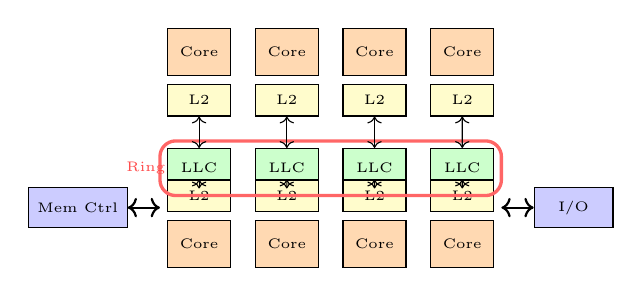
\begin{tikzpicture}[scale=0.45,
    core/.style={draw, fill=orange!30, minimum width=8mm, minimum height=6mm, font=\tiny},
    cache/.style={draw, fill=yellow!20, minimum width=8mm, minimum height=4mm, font=\tiny},
    llc/.style={draw, fill=green!20, minimum width=8mm, minimum height=5mm, font=\tiny},
    ctrl/.style={draw, fill=blue!20, minimum width=10mm, minimum height=5mm, font=\tiny},
    ring/.style={draw, very thick, red!60, rounded corners=2mm}]

% Row 1: 4 cores with L2 cache
\node[core] (c1) {Core};
\node[cache, below=1mm of c1] (l2-1) {L2};
\node[core, right=3mm of c1] (c2) {Core};
\node[cache, below=1mm of c2] (l2-2) {L2};
\node[core, right=3mm of c2] (c3) {Core};
\node[cache, below=1mm of c3] (l2-3) {L2};
\node[core, right=3mm of c3] (c4) {Core};
\node[cache, below=1mm of c4] (l2-4) {L2};

% Row 2: LLC slices
\node[llc, below=4mm of l2-1] (llc1) {LLC};
\node[llc, below=4mm of l2-2] (llc2) {LLC};
\node[llc, below=4mm of l2-3] (llc3) {LLC};
\node[llc, below=4mm of l2-4] (llc4) {LLC};

% Row 3: 4 more cores with L2 cache
\node[core, below=4mm of llc1] (c5) {Core};
\node[cache, above=1mm of c5] (l2-5) {L2};
\node[core, below=4mm of llc2] (c6) {Core};
\node[cache, above=1mm of c6] (l2-6) {L2};
\node[core, below=4mm of llc3] (c7) {Core};
\node[cache, above=1mm of c7] (l2-7) {L2};
\node[core, below=4mm of llc4] (c8) {Core};
\node[cache, above=1mm of c8] (l2-8) {L2};

% Ring interconnect (rectangle around LLC row)
\draw[ring] ([xshift=-2mm, yshift=2mm]llc1.north west) rectangle ([xshift=2mm, yshift=-2mm]llc4.south east);
\node[font=\tiny, red!70] at ([xshift=-6mm]llc1.west) {Ring};

% Memory Controller and I/O on the sides
\node[ctrl, left=5mm of llc1, yshift=-5mm] (mc) {Mem Ctrl};
\node[ctrl, right=5mm of llc4, yshift=-5mm] (io) {I/O};

% Connections
\draw[<->, thin] (l2-1) -- (l2-1 |- llc1.north);
\draw[<->, thin] (l2-2) -- (l2-2 |- llc2.north);
\draw[<->, thin] (l2-3) -- (l2-3 |- llc3.north);
\draw[<->, thin] (l2-4) -- (l2-4 |- llc4.north);
\draw[<->, thin] (l2-5) -- (l2-5 |- llc1.south);
\draw[<->, thin] (l2-6) -- (l2-6 |- llc2.south);
\draw[<->, thin] (l2-7) -- (l2-7 |- llc3.south);
\draw[<->, thin] (l2-8) -- (l2-8 |- llc4.south);

% MC and I/O to ring
\draw[<->, thick] (mc.east) -- ([xshift=-2mm]llc1.west |- mc.east);
\draw[<->, thick] (io.west) -- ([xshift=2mm]llc4.east |- io.west);

\end{tikzpicture}
\end{center}
\footnotesize
Ring interconnect between cores, shared LLC, memory controller, and I/O
\end{columns}
\end{frame}

% Slide: Multi-Socket System
\begin{frame}{Multi-Socket System (NUMA)}
\begin{columns}[T]
\column{0.5\textwidth}
\textbf{Architecture:}
\begin{itemize}
\item Multiple CMP chips per machine
\item Each socket has local memory (NUMA)
\item High-speed point-to-point interconnect
  \begin{itemize}
  \item Intel UPI, AMD Infinity Fabric
  \end{itemize}
\end{itemize}

\vspace{0.3cm}
\textbf{Cache Coherency (ccNUMA):}
\begin{itemize}
\item Shared address space across sockets
\item Directory-based coherency protocol
\item Hardware manages consistency
\end{itemize}

\column{0.5\textwidth}
\begin{center}
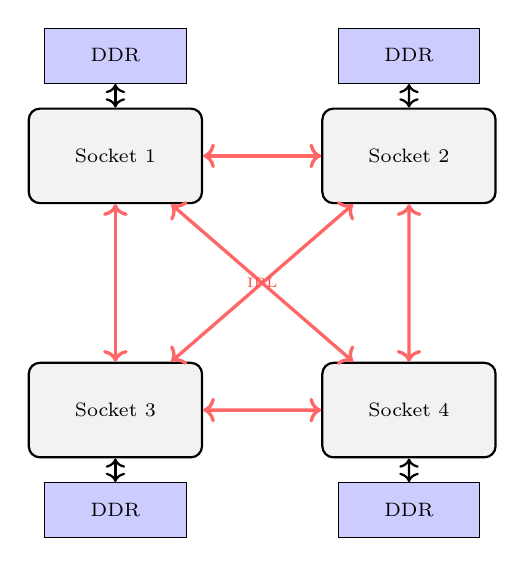
\begin{tikzpicture}[scale=0.6,
    comp/.style={draw, minimum height=7mm, minimum width=12mm, font=\scriptsize, text depth=0.5ex, text height=1.5ex},
    socket/.style={draw, thick, rounded corners, minimum width=2.2cm, minimum height=1.2cm, fill=gray!10, font=\scriptsize},
    mem/.style={comp, fill=blue!20, minimum width=1.8cm}]

% Socket 1 (top-left) - DDR above
\node[socket] (s1) {Socket 1};
\node[mem, above=3mm of s1] (ddr1) {DDR};

% Socket 2 (top-right) - DDR above
\node[socket, right=1.5cm of s1] (s2) {Socket 2};
\node[mem, above=3mm of s2] (ddr2) {DDR};

% Socket 3 (bottom-left) - DDR below
\node[socket, below=2cm of s1] (s3) {Socket 3};
\node[mem, below=3mm of s3] (ddr3) {DDR};

% Socket 4 (bottom-right) - DDR below
\node[socket, right=1.5cm of s3] (s4) {Socket 4};
\node[mem, below=3mm of s4] (ddr4) {DDR};

% IPL connections (fully connected)
\draw[<->, very thick, red!60] (s1) -- (s2);
\draw[<->, very thick, red!60] (s3) -- (s4);
\draw[<->, very thick, red!60] (s1) -- (s3);
\draw[<->, very thick, red!60] (s2) -- (s4);
\draw[<->, very thick, red!60] (s1) -- (s4);
\draw[<->, very thick, red!60] (s2) -- (s3);

% Socket to memory connections
\draw[<->, thick] (s1) -- (ddr1);
\draw[<->, thick] (s2) -- (ddr2);
\draw[<->, thick] (s3) -- (ddr3);
\draw[<->, thick] (s4) -- (ddr4);

\node[font=\tiny, red!70] at ($(s1)!0.5!(s4)$) {IPL};
\end{tikzpicture}
\end{center}
\end{columns}
\end{frame}

% Slide: Server Systems
\begin{frame}{Server Systems}
\begin{columns}[T]
\column{0.55\textwidth}
\textbf{Server systems combine:}
\begin{itemize}
\item \textbf{SMP}: Multiple sockets per motherboard
\item \textbf{CMP}: Multiple cores per socket
\item \textbf{SMT}: Multiple threads per core
\end{itemize}

\vspace{0.3cm}
\textbf{Example: Intel\textsuperscript{\textregistered} Xeon\textsuperscript{\textregistered} E7-8890 V4}
\begin{itemize}
\item SMP: Up to 8 processors per board
\item CMP: 24 cores per processor
\item SMT: 2 threads per core
\item Total: $8 \times 24 \times 2 = 384$ threads
\end{itemize}

\vspace{0.3cm}
\textbf{Blade servers:}
\begin{itemize}
\item Multiple blades per rack
\item Blades connect via network (e.g., InfiniBand\textsuperscript{\textregistered})
\end{itemize}

\column{0.45\textwidth}
\begin{center}
\includegraphics[width=0.9\textwidth]{figures/xeon_e7.jpeg}

\vspace{0.3cm}
\includegraphics[width=0.9\textwidth]{figures/server_blade.jpeg}
\end{center}
\end{columns}
\end{frame}

%%%%%%%%%%%%%%%%%%%%%%%%%%%%%%%%%%%%%%%%%%%%%%%%%%%%%%%%%%%%%%%%%%%%%%%%%%%%%%%
% BACKUP SLIDES
%%%%%%%%%%%%%%%%%%%%%%%%%%%%%%%%%%%%%%%%%%%%%%%%%%%%%%%%%%%%%%%%%%%%%%%%%%%%%%%

\appendix

\begin{frame}
\centering
{\Huge Backup Slides}
\end{frame}

% Backup: Memory Latency Numbers
\begin{frame}{Memory Latency Reference}
\begin{center}
\textbf{Typical Memory Access Latencies}

\vspace{0.5cm}
\begin{tabular}{lrl}
\toprule
\textbf{Level} & \textbf{Latency} & \textbf{Notes} \\
\midrule
L1 Cache & 1--4 cycles & $\sim$1 ns \\
L2 Cache & 10--20 cycles & $\sim$3--7 ns \\
L3 Cache (local) & 30--50 cycles & $\sim$10--20 ns \\
L3 Cache (remote slice) & 50--70 cycles & Mesh/ring traversal \\
\midrule
Local DRAM & 80--150 cycles & $\sim$50--100 ns \\
Remote DRAM (1 hop) & 150--250 cycles & $\sim$100--150 ns \\
Remote DRAM (2 hops) & 200--350 cycles & $\sim$150--250 ns \\
\midrule
NVMe SSD & & $\sim$10--100 $\mu$s \\
HDD & & $\sim$5--10 ms \\
\bottomrule
\end{tabular}
\end{center}

\vspace{0.3cm}
\footnotesize
\textbf{Note:} Actual latencies vary by CPU architecture, memory speed, and system configuration.
\end{frame}

% Backup: Real System Topology - Part 1
\begin{frame}{Real System Topology (Part 1)}
\begin{columns}[T]
\column{0.46\textwidth}
\begin{center}
\vspace{-8mm}
\includegraphics[width=\textwidth,height=0.85\textheight,keepaspectratio]{figures/topo.png}
\end{center}

\column{0.54\textwidth}
\textbf{1. Two-Socket NUMA System}
\begin{itemize}
\item 2 Packages (CPU sockets)
\item 2 NUMA nodes (125GB + 126GB)
\item Each package: 28 cores
\item Total: 56 physical cores
\end{itemize}

\vspace{0.5cm}
\textbf{2. Hyperthreading (SMT)}
\begin{itemize}
\item Each core has 2 PUs (processing units)
\item PU = hardware thread
\item Total: 112 logical processors
\item PU IDs interleaved\\(P\#0, P\#56, P\#2, P\#58...)
\end{itemize}
\end{columns}
\end{frame}

% Backup: Real System Topology - Part 2
\begin{frame}{Real System Topology (Part 2)}
\begin{columns}[T]
\column{0.46\textwidth}
\begin{center}
\vspace{-8mm}
\includegraphics[width=\textwidth,height=0.85\textheight,keepaspectratio]{figures/topo.png}
\end{center}

\column{0.54\textwidth}
\textbf{3. Cache Hierarchy}
\begin{itemize}
\item \textcolor{red}{Private} per core:
  \begin{itemize}
  \item L1i: 32KB (instruction)
  \item L1d: 48KB (data)
  \item L2: 2MB
  \end{itemize}
\item \textcolor{blue}{Shared} per package:
  \begin{itemize}
  \item L3: 53MB (all 28 cores)
  \end{itemize}
\end{itemize}

\vspace{0.5cm}
\textbf{4. I/O Device Locality}
\begin{itemize}
\item PCI devices attached to specific packages
\item Package 0: Ethernet, VGA, SATA, RAID
\item Package 1: High-speed Ethernet (mlx5)
\item Accessing devices $\rightarrow$ prefer local memory!
\end{itemize}

\vspace{0.3cm}
\textbf{Tip:} Pin network threads to Package 1 cores for best mlx5 performance!
\end{columns}
\end{frame}

% Backup: Mesh Routing (hidden)
\iffalse
\begin{frame}{Mesh Routing}
\begin{columns}[T]
\column{0.55\textwidth}
\textbf{Simple XY Routing Algorithm:}
\begin{enumerate}
\item Packet originates at source tile
\item Enters fabric via local mesh stop
\item \textbf{First: Route vertically} (north or south)
\begin{itemize}
\item Takes shortest path on vertical ring
\item Continues until destination row reached
\end{itemize}
\item \textbf{Then: Route horizontally} (east or west)
\begin{itemize}
\item Switches to horizontal ring
\item Continues to destination column
\end{itemize}
\item Exits fabric via destination mesh stop
\end{enumerate}

\vspace{0.2cm}
\textbf{Note:} Return path may be different (asymmetric)

\column{0.45\textwidth}
\begin{center}
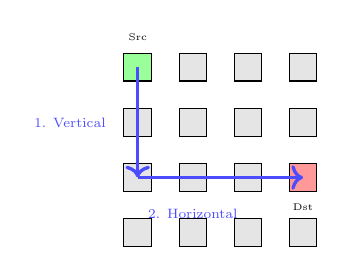
\begin{tikzpicture}[scale=0.7, transform shape,
    node/.style={draw, fill=gray!20, minimum size=0.5cm, inner sep=0pt},
    src/.style={node, fill=green!40},
    dst/.style={node, fill=red!40},
    path/.style={->, very thick, blue!70}
]
% 4x4 grid of nodes
\foreach \x in {0,1,2,3} {
    \foreach \y in {0,1,2,3} {
        \node[node] (n\x\y) at (\x, \y) {};
    }
}
% Source and destination
\node[src] at (0,3) {};
\node[dst] at (3,1) {};
\node[font=\tiny, above=0.1cm of n03] {Src};
\node[font=\tiny, below=0.1cm of n31] {Dst};

% Path: vertical first, then horizontal
\draw[path] (n03.center) -- (n01.center);
\draw[path] (n01.center) -- (n31.center);

% Labels
\node[font=\scriptsize, left=0.2cm of n02, blue!70] {1. Vertical};
\node[font=\scriptsize, below=0.2cm of n11, blue!70] {2. Horizontal};
\end{tikzpicture}
\end{center}

\vspace{0.2cm}
\textbf{Benefits:}
\begin{itemize}
\item Deadlock-free routing
\item Predictable latency
\item Simple hardware
\end{itemize}
\end{columns}
\end{frame}
% Slide: DDR-SDRAM
\begin{frame}{DDR-SDRAM}
\textbf{2n-prefetch architecture doubles data rate}

\vspace{0.2cm}
\begin{columns}[T]
\column{0.58\textwidth}
\textbf{How it works:}
\begin{itemize}
\item DRAM core operates at same speed as SDR
\item Internal bus: 2$\times$ wider than external
\item Data transferred twice per clock:
  \begin{itemize}
  \item Rising edge: lower half (0:n-1)
  \item Falling edge: upper half (n:2n-1)
  \end{itemize}
\item Example: 200MHz clock = 400MT/s
\end{itemize}

\vspace{0.2cm}
\textbf{Reduced power:} 2.5V vs. 3.3V in SDR

\column{0.38\textwidth}
\vspace{0.2cm}
\begin{center}
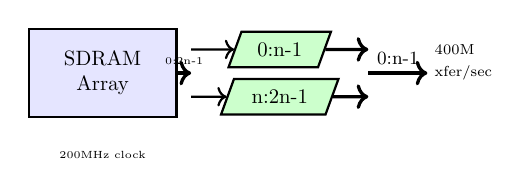
\begin{tikzpicture}[scale=0.75, transform shape]
  % SDRAM Array
  \node[draw, thick, minimum width=2.5cm, minimum height=1.5cm, fill=blue!10, align=center] (array) at (0,0) {SDRAM\\Array};

  % Two multiplexers
  \node[draw, thick, trapezium, trapezium left angle=70, trapezium right angle=110, minimum width=1cm, minimum height=0.6cm, fill=green!20] (mux1) at (3,0.4) {0:n-1};
  \node[draw, thick, trapezium, trapezium left angle=70, trapezium right angle=110, minimum width=1cm, minimum height=0.6cm, fill=green!20] (mux2) at (3,-0.4) {n:2n-1};

  % Internal bus
  \draw[->, very thick] (array.east) -- node[above, font=\tiny] {0:2n-1} (1.5,0);
  \draw[->, thick] (1.5,0.4) -- (mux1.west);
  \draw[->, thick] (1.5,-0.4) -- (mux2.west);

  % Output
  \draw[->, very thick] (mux1.east) -- (4.5,0.4);
  \draw[->, very thick] (mux2.east) -- (4.5,-0.4);
  \draw[->, very thick] (4.5,0) -- node[above, font=\small] {0:n-1} (5.5,0);
  \node[right, font=\scriptsize] at (5.5,0.4) {400M};
  \node[right, font=\scriptsize] at (5.5,0) {xfer/sec};

  % Clock label
  \node[below, font=\tiny] at (0,-1.2) {200MHz clock};
\end{tikzpicture}
\end{center}
\end{columns}
\end{frame}
% Slide: DDR SDRAM Timing
\begin{frame}{DDR SDRAM Timing}
\vspace{-0.2cm}
\begin{center}
\begin{tikztimingtable}[
  timing/slope=0.15,
  timing/coldist=0.35cm,
  xscale=1.7,
  timing/rowdist=0.6cm,
  timing/name/.style={font=\small}
]
  clock & L H L H L H L H L H L H L H L H L H L H L H L H L H\\
  cmd   & 2D{\textcolor{cyan}{ACT}} 4U 2D{\textcolor{cyan}{RD}} 2U 2D{\textcolor{blue}{ACT}} 4U 2D{\textcolor{blue}{RD}} 2U 2D{\textcolor{cyan}{ACT}} 4U \\
  \\
  Bank  & 2D{\textcolor{cyan}{Bank 0}} 4U 2D{\textcolor{cyan}{Bank 0}} 2U 2D{\textcolor{blue}{Bank 1}} 4U 2D{\textcolor{blue}{Bank1}} 2U 2D{\textcolor{cyan}{Bank 0}} 4U \\
  Addr  & 2D{\textcolor{cyan}{Row i}} 4U 2D{\textcolor{cyan}{Col j}} 2U 2D{\textcolor{blue}{Row l}} 4U 2D{\textcolor{blue}{Col j}} 2U 2D{\textcolor{cyan}{Row m}} 4U \\
  \\
  Data  & 12U D{\textcolor{cyan}{j}} D{\textcolor{cyan}{+1}} D{\textcolor{cyan}{+2}} D{\textcolor{cyan}{+3}} 6U D{\textcolor{cyan!50}{n}} D{\textcolor{cyan!50}{+1}} D{\textcolor{cyan!50}{+2}} D{\textcolor{cyan!50}{+3}} \\
  \extracode
    % Vertical grid lines
    \begin{scope}[gray!30, thin]
      \foreach \x in {0,2,...,24} {
        \draw[dashed] (\x+0.15,0.5) -- (\x+0.15,-12);
      }
    \end{scope}
    % Timing annotations
    \begin{scope}[>=stealth, font=\scriptsize]
      % tRCD
      \draw[<->,thick] (7.15,-3) -- node[midway, fill=white, inner sep=1pt] {$t_{\text{RCD}}>20$ns} (1.15,-3);
      \draw (7.15,-2) -- (7.15,-3);
      \draw (1.15,-2) -- (1.15,-4);
      % tRC
      \draw[<->,thick] (1.15,-4) -- node[midway, fill=white, inner sep=1pt] {$t_{\text{RC}}>70$ns} (21.15,-4);
      \draw (21.15,-2) -- (21.15,-4);
      % tRRD
      \draw[<->,thick] (11.15,-3) -- node[midway, fill=white, inner sep=1pt] {$t_{\text{RRD}}>20$ns} (21.15,-3);
      \draw (11.15,-2) -- (11.15,-3);
      % CL
      \draw[<->,thick] (12.15,-9.5) -- node[midway, fill=white, inner sep=1pt] {CL=2} (7.15,-9.5);
      \draw (7.15,-10) -- (7.15,-8);
      \draw (12.15,-9) -- (12.15,-11);
    \end{scope}
\end{tikztimingtable}
\end{center}

\vspace{-0.3cm}
\textbf{Key timing parameters:}
\begin{itemize}
\item $\mathbf{t_{\text{RCD}}}$: Same as SDR SDRAM
\item $\mathbf{t_{\text{RC}}}$: Same as SDR SDRAM
\item $\mathbf{t_{\text{RRD}}}$: Same as SDR SDRAM
\item \textbf{Burst length = 4:} Each READ transfers 4 consecutive locations (both edges)
\end{itemize}
\end{frame}
% Slide: DRAM Controller Performance
\begin{frame}{DRAM Controller: Performance Considerations}
\textbf{Cache line granularity:}
\begin{itemize}
\item All reads/writes operate on full cache lines (64 bytes)
\item Even if you only need 1 byte, entire line is transferred
\end{itemize}

\vspace{0.3cm}
\textbf{Write buffering:}
\begin{itemize}
\item Writes complete when data enters controller's write buffer (not DRAM!)
\item Buffer flushed to DRAM later $\rightarrow$ low write latency
\item Out-of-order scheduler reorders for maximum efficiency
\end{itemize}

\vspace{0.3cm}
\textbf{Partial writes (performance killer):}
\begin{itemize}
\item \textbf{Problem:} Writing $<$64 bytes requires Read-Modify-Write:
  \begin{enumerate}
  \item Read full cache line from DRAM
  \item Modify only the bytes you want to change
  \item Write full cache line back to DRAM
  \end{enumerate}
\item \textbf{Common causes:} Non-cacheable I/O device writes, unaligned accesses
\item \textbf{Software fix:} Buffer small writes into full cache line writes
\end{itemize}

\vspace{0.2cm}
\textbf{Takeaway:} Access memory in cache-line-sized chunks for best performance
\end{frame}
% Slide 6: Modern Examples
\begin{frame}{Modern CPU Examples}
\begin{center}
\vspace{-3mm}
\footnotesize
\begin{tabular}{l|c|c|c|c}
\toprule
\textbf{CPU} & \textbf{Cores/Die} & \textbf{Dies/Pkg} & \textbf{Interconnect} & \textbf{Notes} \\
\midrule
Intel Core i9-13900K & 24 (8P+16E) & 1 & Ring + Fabric & Monolithic \\
Intel Xeon Platinum & up to 40 & 1 & Mesh & Monolithic, tiles \\
\midrule
AMD Ryzen 9 7950X & 16 & 2 CCD + 1 IOD & IF (intra \& inter) & Chiplet \\
AMD EPYC 9654 & 96 & 12 CCD + 1 IOD & IF & Massive chiplet \\
\midrule
Apple M2 Ultra & 24 & 2 & UltraFusion & Die-to-die bridge \\
\midrule
Intel Sapphire Rapids & up to 60 & 4 & EMIB bridges & Multi-tile \\
\bottomrule
\end{tabular}
\end{center}

\vspace{1mm}
\begin{columns}[T]
\column{0.4\textwidth}
\textbf{Monolithic Advantages:}
\begin{itemize}
\item Lower latency
\item Simpler software model
\item No die-to-die overhead
\end{itemize}

\column{0.6\textwidth}
\textbf{Multi-Die Advantages:}
\begin{itemize}
\item Higher core counts
\item Better yields
\item Mix-and-match configs, reusable components
\end{itemize}
\end{columns}

\vspace{1mm}
\textbf{Software must adapt for optimal performance!}
\end{frame}
% Slide 3: Ring Interconnect Details
\begin{frame}{Ring Interconnect: How It Works}
\begin{columns}[T]
\column{0.5\textwidth}
\textbf{Ring Architecture:}
\begin{itemize}
\item Bidirectional rings (clockwise + counter-clockwise)
\item Each "stop" contains:
  \begin{itemize}
  \item CPU core
  \item L3 cache slice
  \item Connection logic
  \end{itemize}
\item Messages take shortest path
\item Typically 32-byte data ring
\end{itemize}

\vspace{0.3cm}
\textbf{Why Rings Work Well (up to a point):}
\begin{itemize}
\item Simple to implement
\item Predictable latency
\item Good bandwidth for small core counts
\item Power efficient
\end{itemize}

\column{0.5\textwidth}
\begin{center}
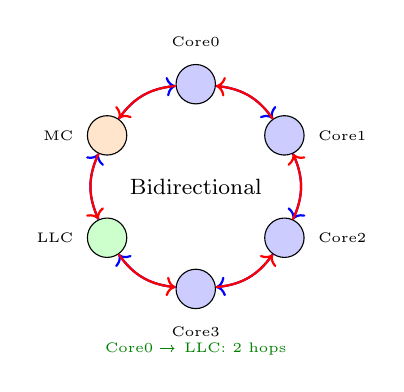
\begin{tikzpicture}[
    stop/.style={draw, circle, fill=blue!20, minimum size=0.5cm, inner sep=1pt, font=\tiny}
]
% Ring stops positioned explicitly
\node[stop] (s0) at (90:1.3) {};
\node[font=\tiny, above=0.1cm of s0] {Core0};
\node[stop] (s1) at (30:1.3) {};
\node[font=\tiny, right=0.05cm of s1] {Core1};
\node[stop] (s2) at (-30:1.3) {};
\node[font=\tiny, right=0.05cm of s2] {Core2};
\node[stop] (s3) at (-90:1.3) {};
\node[font=\tiny, below=0.1cm of s3] {Core3};
\node[stop, fill=green!20] (s4) at (-150:1.3) {};
\node[font=\tiny, left=0.05cm of s4] {LLC};
\node[stop, fill=orange!20] (s5) at (150:1.3) {};
\node[font=\tiny, left=0.05cm of s5] {MC};

% Clockwise ring (blue, inner)
\draw[->, thick, blue] (s0) to[bend left=25] (s1);
\draw[->, thick, blue] (s1) to[bend left=25] (s2);
\draw[->, thick, blue] (s2) to[bend left=25] (s3);
\draw[->, thick, blue] (s3) to[bend left=25] (s4);
\draw[->, thick, blue] (s4) to[bend left=25] (s5);
\draw[->, thick, blue] (s5) to[bend left=25] (s0);

% Counter-clockwise ring (red, outer)
\draw[->, thick, red] (s0) to[bend right=25] (s5);
\draw[->, thick, red] (s5) to[bend right=25] (s4);
\draw[->, thick, red] (s4) to[bend right=25] (s3);
\draw[->, thick, red] (s3) to[bend right=25] (s2);
\draw[->, thick, red] (s2) to[bend right=25] (s1);
\draw[->, thick, red] (s1) to[bend right=25] (s0);

\node[font=\footnotesize] at (0,0) {Bidirectional};

% Example path annotation
\node[font=\tiny, green!50!black, below=0.3cm of s3] {Core0 → LLC: 2 hops};
\end{tikzpicture}
\end{center}

\textbf{Limitations:} Shared bandwidth, latency grows with cores, not for >10-12 cores
\end{columns}
\end{frame}
\fi

\end{document}